\documentclass{report}

\usepackage[backend=bibtex]{biblatex}
\usepackage{graphicx}
\usepackage{listings}
\usepackage{lmodern}
\usepackage{minted}
\usepackage{multirow}
\usepackage{subcaption}
\usepackage{tabularx}
\usepackage{tcolorbox}
\usepackage[utf8]{inputenc}
\usepackage{hyperref}
\usepackage[toc]{glossaries}

\lstset{basicstyle=\ttfamily,
	literate=
	{á}{{\'a}}1 {é}{{\'e}}1 {í}{{\'i}}1 {ó}{{\'o}}1 {ú}{{\'u}}1
	{Á}{{\'A}}1 {É}{{\'E}}1 {Í}{{\'I}}1 {Ó}{{\'O}}1 {Ú}{{\'U}}1
	{à}{{\`a}}1 {è}{{\`e}}1 {ì}{{\`i}}1 {ò}{{\`o}}1 {ù}{{\`u}}1
	{À}{{\`A}}1 {È}{{\'E}}1 {Ì}{{\`I}}1 {Ò}{{\`O}}1 {Ù}{{\`U}}1
	{ä}{{\"a}}1 {ë}{{\"e}}1 {ï}{{\"i}}1 {ö}{{\"o}}1 {ü}{{\"u}}1
	{Ä}{{\"A}}1 {Ë}{{\"E}}1 {Ï}{{\"I}}1 {Ö}{{\"O}}1 {Ü}{{\"U}}1
	{â}{{\^a}}1 {ê}{{\^e}}1 {î}{{\^i}}1 {ô}{{\^o}}1 {û}{{\^u}}1
	{Â}{{\^A}}1 {Ê}{{\^E}}1 {Î}{{\^I}}1 {Ô}{{\^O}}1 {Û}{{\^U}}1
	{œ}{{\oe}}1 {Œ}{{\OE}}1 {æ}{{\ae}}1 {Æ}{{\AE}}1 {ß}{{\ss}}1
	{ű}{{\H{u}}}1 {Ű}{{\H{U}}}1 {ő}{{\H{o}}}1 {Ő}{{\H{O}}}1
	{ç}{{\c c}}1 {Ç}{{\c C}}1 {ø}{{\o}}1 {å}{{\r a}}1 {Å}{{\r A}}1
	{€}{{\euro}}1 {£}{{\pounds}}1 {«}{{\guillemotleft}}1
	{»}{{\guillemotright}}1 {ñ}{{\~n}}1 {Ñ}{{\~N}}1 {¿}{{?`}}1
}

\newcommand{\code}[1]{\textsf{\ttfamily #1}}
\newcommand{\notefor}[1]{\hfill\textbf{\textit{#1}}}
\renewcommand{\glstextformat}[1]{\textbf{#1}}
\addbibresource{Rtutorial.bib}
\makenoidxglossaries

\newglossaryentry{dv}{name={discrete variable}, plural={discrete variables}, description={A variable that refers to categorical data (ex. color of eyes), as opposed to continuous data (ex. height in mm)}}

\newglossaryentry{cv}{name={continuous variable}, plural={continuous variables}, description={A variable that refers to continuous data, i.e. that can take on an infinite number of values (ex. height in mm), as opposed to categorical data (ex. color of eyes)}}

\newglossaryentry{ov}{name={ordinal variable}, plural={ordinal variables}, description={A qualitative variable where the values can be ordered (ex. small, medium, large)}}

\newglossaryentry{qtv}{name={quantitative variable}, plural={quantitative variables}, description={A variable that is measured with numbers (ex. number of cases, height in mm)}}

\newglossaryentry{qlv}{name={qualitative variable}, plural={qualitative variables}, description={A variable that is recorded with words rather than numbers (ex. color of eyes, state of mind)}}

\newglossaryentry{depv}{name={dependent variable}, plural={dependent variables}, description={The "explained" variable in a relationship, the one we try to understand as a consequence of another factor. For example, when studying the effect of smoking on lung cancer, lung cancer is the dependent variable.}}

\newglossaryentry{indv}{name={independent variable}, plural={independent variables}, description={The "explaining" variable in a relationship, the one that drives a phenomena. For example, when trying to understand the causes of diabetes, body mass index would be an independent variable.}}

\author{Myriam Luce}
\title{Statistics with R: a hands-on approach}

\begin{document}
\maketitle
\tableofcontents

\chapter{Data review}
	\section{Possibly interesting extra tidbits}
	In the making of this tutorial, I used several tools that you might like to access as well. Being the tedium-averse programmer I am, I use a reference manager program, in my case Zotero. You can find the full bibliography for this project, including a few entries that did not make it into the references section here because I did not cite them, at \href{https://www.zotero.org/groups/2223910/r_tutorial}{the Zotero project page}.
	
	I also want to point out \href{https://github.com/awesomedata/awesome-public-datasets}{awesome-public-datasets}, where I foraged for the examples in this tutorial. It has several interesting datasets in the public health domain.
	
	Finally, this tutorial is not necessarily intended to be done in order. In particular, section~\ref{sec:data-import} should be read as needed, rather than all the beginning. Not only the section on tidying up data might be boring as a first subject on R, but it's also unlikely to make much sense without some hands-on experience using the software. However, it seemed to make sense to keep all things R together, to make it easier to find again later, when the reader encounters the unavoidable data QA issue.

	\section{Variables}
	When ``doing science'', you will be taking measurements, usually in the hopes of understanding a phenomena often in the shape of a relationship between things you are measuring. When working with this data, the nature of the things you measure (\emph{variables}) will influence the presentation and analysis that are appropriate.
	
	A \gls{qlv} refers to categories, or a variable recorded with words, as opposed to a \gls{qtv}, which is measured with numbers. Examples of qualitative variables would include US state, restaurant chains and college major. Quantitative variables could be time to execute a task, waist circumference, disease rate or spending amounts.
	
	R refers to \glspl{qlv} as \emph{factors}. \Glspl{qlv} can further be divided into non ordinal and \glspl{ov}, depending on whether there is a natural order among the categories. For example, dog breed (chihuahua, husky, labrador) is a non ordinal variable, whereas level of satisfaction (dissatisfied, neutral, satisfied) is ordinal.
	
	\Glspl{qtv} are either \glspl{dv}, where measurements are done in integers, or \glspl{cv}, where they come in real numbers (you could get an infinity of decimals with a theoretical instrument of infinite precision). \Glspl{dv} could be number of children, cancer deaths, or wedding age. \Glspl{cv} include temperature, blood sugar level, and weight.
	
	Furthermore, when studying variables in relationship with one another, changes in a \gls{depv} are driven or explained by an \gls{indv}. Typically, this means the ``x'' axis of a graph will be the \gls{indv}, while the ``y'' axis will be the \gls{depv}.
	
	\section{Gotchas}
		\subsection{Tidy data}\label{subsec:gotcha_tidy}
		When working with data in R, analysis will be easier if your data is \emph{tidy}, that is, each column in your data set contains one and only one variable. Or, more completely:
		\begin{enumerate}
			\item Each variable is in its own column
			\item Each observation is in its own row
			\item Each value is in its own cell
		\end{enumerate}
		
		(Garrett Grolemund gives an excellent introduction to the subject \cite{tidy}.)
		
		For example, in a cancer dataset that we will use later, the original data is presented as in table \ref{table:cancer}. Here, we have four variables: cancer type, sex, number of cases, and number of deaths. While the first column is one and only one variable, the other columns mix sex with number of cases or sex with number of deaths. If you would like to analyze deaths by sex or cases per cancer type, some data manipulation will be necessary to combine the relevant columns.
		\begin{table}[h]
			\centering
			\begin{tabular}{|c|c|c|c|c|}
				\hline 
				\multirow{2}{*}{Cancer Type} & \multicolumn{2}{c|}{Cases}  & \multicolumn{2}{c|}{Deaths} \\ 
				& Male & Female & Male & Female \\  \hline 
				... &  ... & ...  & ...  & ...  \\ \hline 
			\end{tabular} 
			\caption{Cancer data set format.}
			\label{table:cancer}
		\end{table}

		If you keep your data tidy, R can usually do the combining for you, if you know how to ask nicely. As such, it is recommended that the first thing you do after successfully importing data into R is to verify it is tidy. Tools to divide or merge columns will be discussed in section \ref{sec:data-import}.
	
		\subsection{Correlation is not causation, or of the importance of DoE}
		DoE refers to design of experiments. The common trope that ``correlation is not causation'' refers to the fact that because two variables vary together does not necessarily mean that one causes the other to change; for instance, they might both be responding to a common cause, when it's not just plain old coincidence. My personal favorite exemplification of ``correlation is not causation'' is that the divorce rate in Maine correlates with the per capita consumption of margarine \cite{vigen}.
	
		To distinguish between correlation and causation with certainty, a controlled experiment must be run. Depending on the phenomena studied, this might mean using a control group, a placebo, or directly controlling environmental conditions. For example, to determine the effect of low oxygen concentration in water on cod growth, several tanks can be set up where individual cods are randomly distributed and where oxygen levels are controlled. If you were to simply measure oxygen levels in water and cod growth at different locations and subsequently find a correlation between the two, you couldn't tell for certain whether the difference is due to oxygen levels, or another factor like water temperature, or even the fact that cod compete with one another and that the runts, who would grow slower anyway, end up pushed into less desirable low-oxygen environments. Of course, sometimes running a controlled experiment is not feasible for practical reasons (one can't control amount of natural sunlight, for example) or ethical reasons (having an untreated control group of people with a serious condition, when a potentially life-saving treatment might exist, is questionable).
	
		When dealing with humans, to determine whether medication has a positive effect on an health issue, the health issue can be measured for a group who took the medication (treatment group), a group who took a placebo, and a group who took no medication at all (control group). In humans, particular effort must be placed on controlling or measuring the placebo effect, for the test subjects as well as the professionals. A recent spectacular example is the recommendation to abandon arthroscopic surgeries for knee pain because it did not show better results than physical therapy in randomized trials, despite it being the most common orthopaedic procedure in several countries \cite{knee}.
	
		Where experimental design is concerned, key factors are randomization, blocking, and replication. If terms like Completely Randomized Design, Latin Squares or Factorial Design are not familiar, I would recommend investing some time into learning the basics of experimental design before embarking in an experiment, in the interest of avoiding some common and easily remedied mistakes (\cite{doe} appears to be a well-rounded textbook ).

\chapter{Unavoidable R before we begin}
	Despite the title, this chapter is not meant to be read from start to finish before you get to the other chapters. First, a long text about programming quirks can get pretty sleep-inducing. Second, the concerns addressed will probably not resonate much with you unless you've personally encountered this problem before, so the information retention is likely to be low.
	
	That being said, the three first sections (\ref{sec:packages}, \ref{sec:types}, \ref{sec:access}) should probably be read right now if you are not familiar with R at all. The other ones are referenced later in the text when they are relevant and can be read at that time.

	\section{Packages}\label{sec:packages}
	R \cite{R} should be relatively straightforward to install: download and execute, follow the wizard instructions.

	Where things get a bit more complicated is when it comes to packages. While the basic R program has a lot of functions built-in, there will come a time when you will need something that is not offered out of the box. Thankfully, R has a very dynamic community with a ton of packages. For instance, a very popular package to produce figures is \code{ggplot2}. Let's install it to see how packages are managed in R.

	First off, to install packages in R, you will need to launch it as an administrator. If you don't, you will get the rather unhelpful message shown in figure~\ref{fig:unhelpful}. To launch with administrator rights, right-click on your R launcher and find the option ``Run as administrator''. How to do so from the Windows 10 start menu is shown in figure~\ref{fig:admin}. (As a note, you should launch as administrator \emph{only} when installing packages, as opposed to modifying your shortcut to always launch as administrator.)
	\begin{figure}[h]
		\centering
		\begin{minipage}{.475\textwidth}
			\centering
			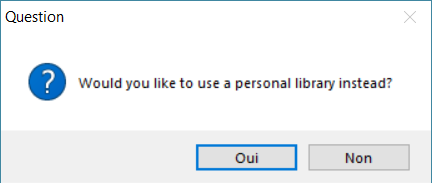
\includegraphics[width=.8\linewidth]{unhelpful.png}
			\caption{Error message displayed by R if trying to install packages without administrator rights.}
			\label{fig:unhelpful}
		\end{minipage}
		\hfill
		\begin{minipage}{.475\textwidth}
			\centering
			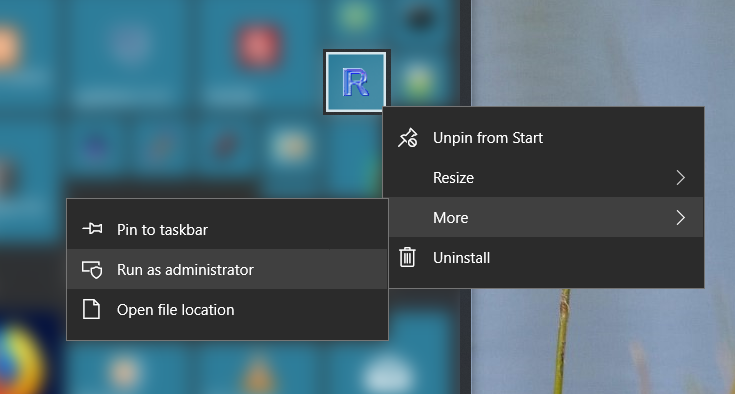
\includegraphics[width=.8\linewidth]{admin.png}
			\caption{How to launch R with administrative rights.}
			\label{fig:admin}
		\end{minipage}
	\end{figure}

	Now that R is launched as administrator, you can install \code{ggplot2} using either the convenient Packages menu or the command line if you're that hardcore. Personally I use the menu; after choosing a mirror (different mirrors offer different packages; Canada NS has a wide selection and is vaguely geographically close), you can select your desired package and hit ``install'', as shown in figure~\ref{fig:install}. Then you only need to wait until R is done doing its thing. If all the lines say ``successfully unpacked'', all good; otherwise, an error has occurred and you will have to decipher the message to figure out how to remedy the situation. (If you run into any trouble, I would first recommend updating to the latest release of R.)
	\begin{figure}[h]
		\centering
		\begin{subfigure}[b]{0.475\textwidth}
			\centering
			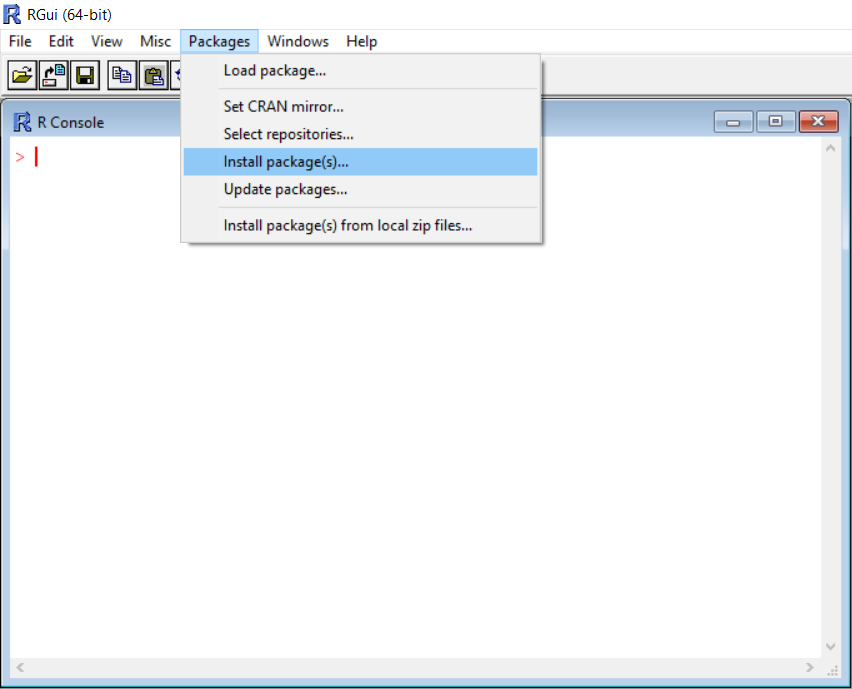
\includegraphics[width=\textwidth]{menu.png}
			\caption{Packages menu in R Gui.}
			\label{fig:menu}
		\end{subfigure}
		\hfill
		\begin{subfigure}[b]{0.475\textwidth}
			\centering
			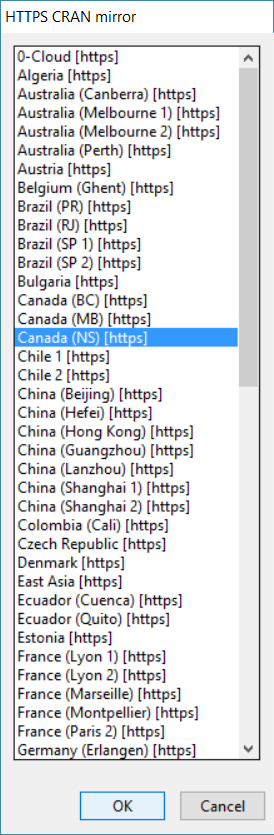
\includegraphics[height=5cm]{mirror.png}
			\caption{List of mirrors.}
			\label{fig:packages}
		\end{subfigure}
		\vskip\baselineskip
		\begin{subfigure}[b]{0.475\textwidth}
			\centering
			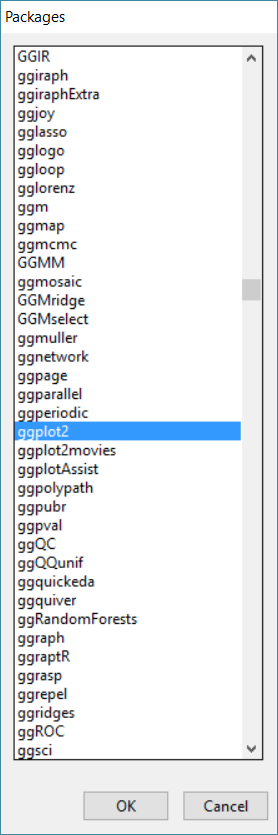
\includegraphics[height=5cm]{packages.png}
			\caption{List of packages.}
			\label{fig:mirror}
		\end{subfigure}
		\hfill
		\begin{subfigure}[b]{0.475\textwidth}
			\centering
			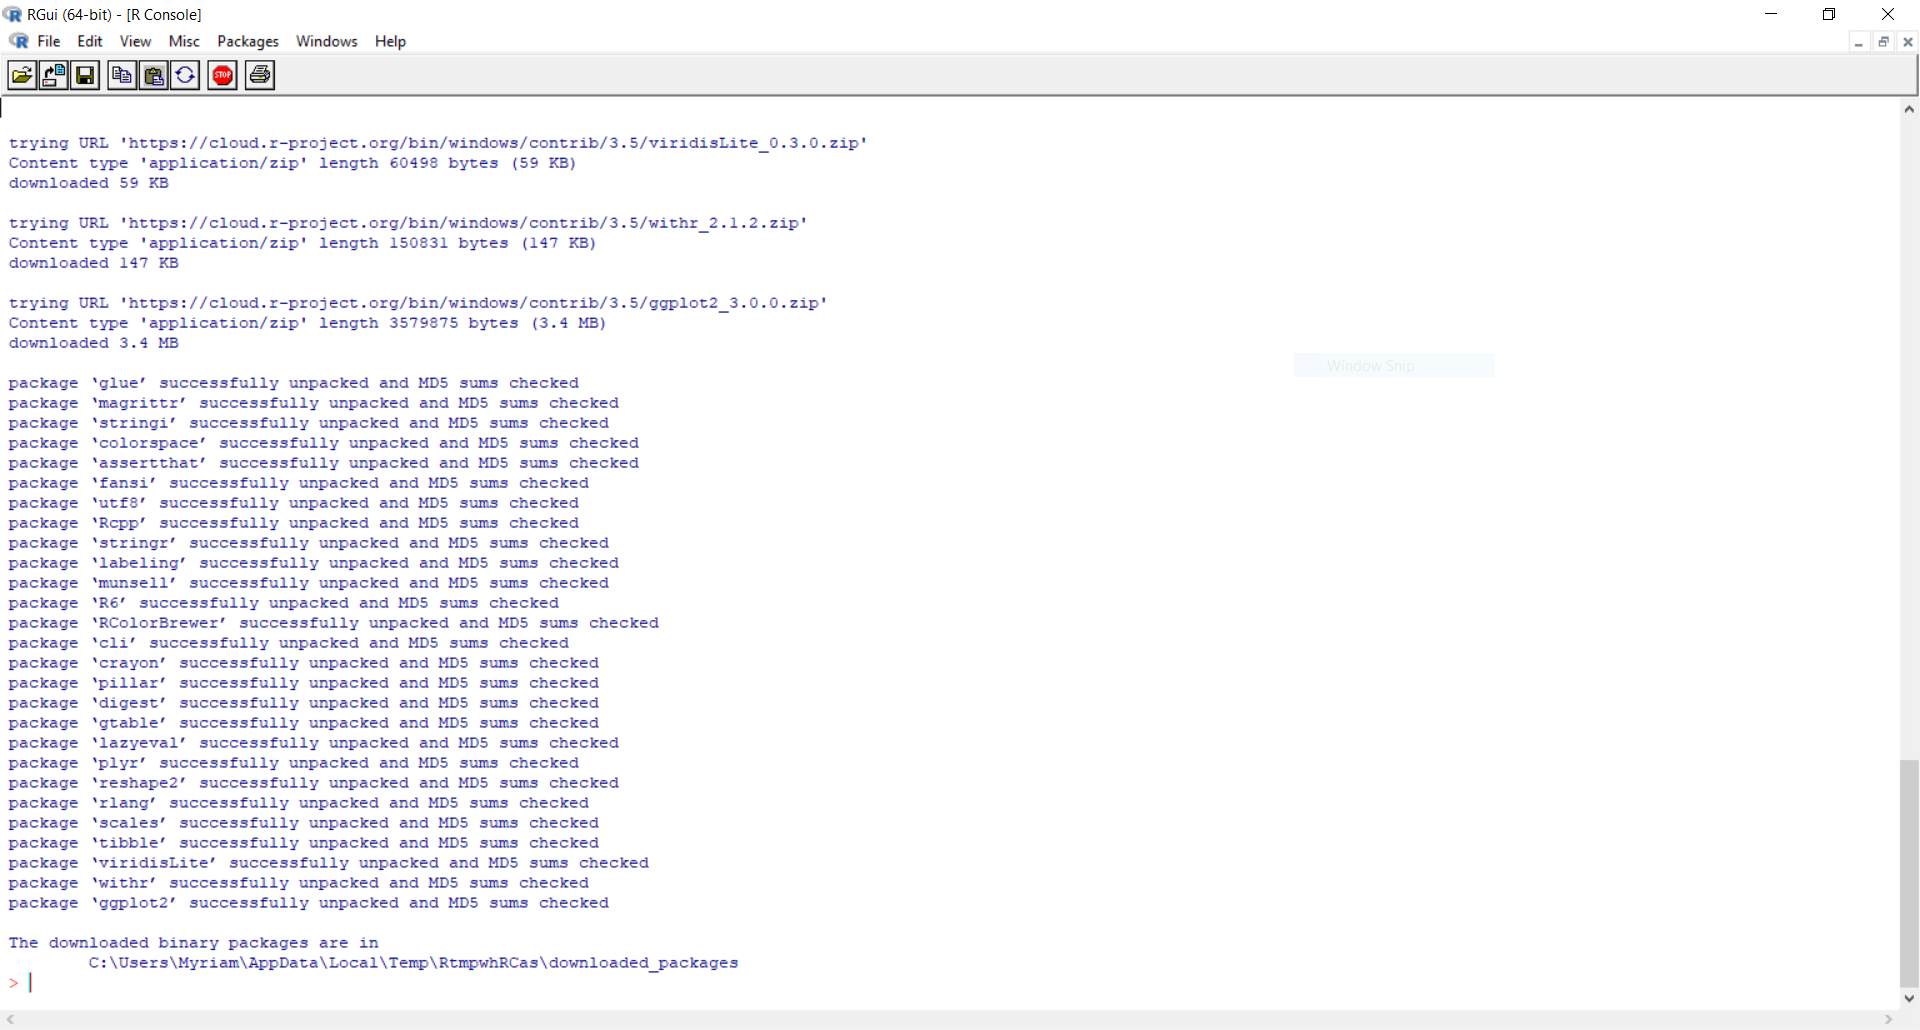
\includegraphics[width=\textwidth]{installed.png}
			\caption{All successfully unpacked: successful installation.}
			\label{fig:installed}
		\end{subfigure}
		\caption{Package installation process.}
		\label{fig:install}
	\end{figure}

	Note that installing a package is not enough to use it; you must also load it. Again this can be done either from the menu or with the command line, as shown in figure~\ref{fig:load}. This operation must be repeated \emph{every time} you restart R.
	\begin{figure}[h]
		\centering
		\begin{subfigure}[t]{0.475\textwidth}
			\centering
			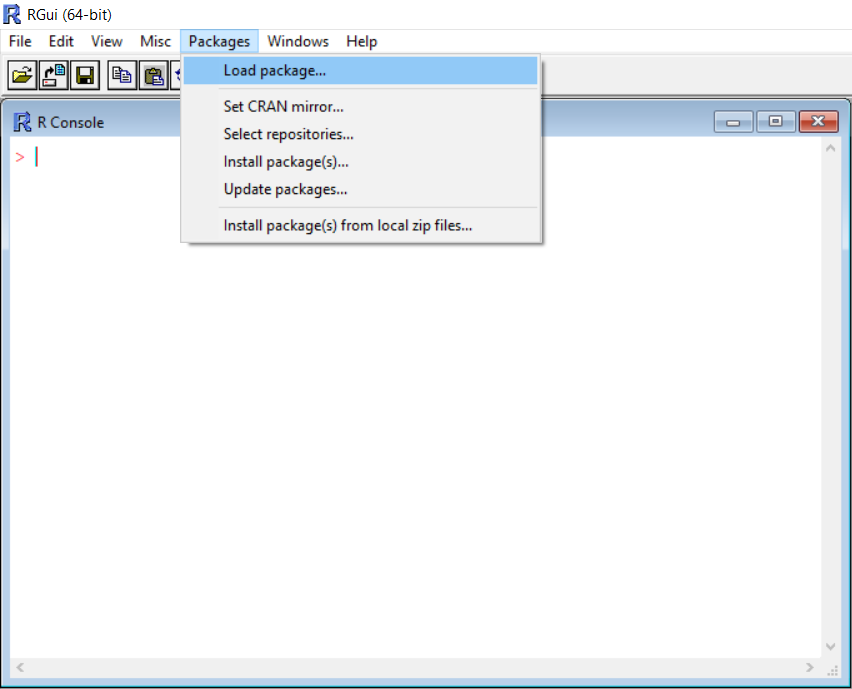
\includegraphics[width=\textwidth]{load.png}
			\caption{Packages menu in R Gui.}
			\label{fig:loadmenu}
		\end{subfigure}
		\hfill
		\begin{subfigure}[t]{0.475\textwidth}
			\centering
			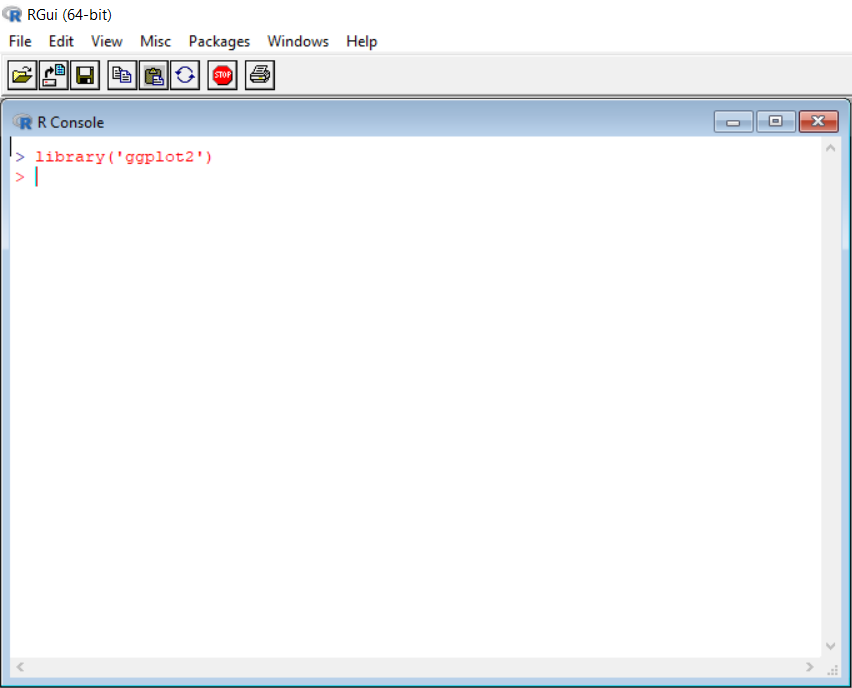
\includegraphics[width=\textwidth]{cli.png}
			\caption{Command to load a package in R Gui.}
			\label{fig:cli}
		\end{subfigure}
		\caption{Loading packages in R.}
		\label{fig:load}
	\end{figure}

	Now let's say that \code{ggplot2} becomes your favoritest package in the whole world and you end up using it every day. After a week or so you will probably be very annoyed having to reload the package every time you open R. You can add packages to be loaded automatically in either of two files: \code{Rprofile.site} or \code{.Rprofile}. \code{Rprofile.site} is located in your R installation folder in the etc folder and is always executed. \code{.Rprofile} is located in the user home folder and is applied after the changes made by \code{Rprofile.site}. As the appropriate location to put \code{.Rprofile} seems to change from R version to version, I will showcase the \code{Rprofile.site} here. At the bottom of the file, add the following:
	\begin{minted}[breaklines]{R}
.First <- function(){
	library('ggplot2')
	# other libraries go here
}
	\end{minted}

	\section{Types}\label{sec:types}
	While relatively accessible as far as programming languages go, R is still a programming language. As such, it has a few concerns that, while painful for the non-programmers among us, are useful tools to diagnose problems, typically when importing data that has not been properly QA'd or when a function refuses to compute because the input is in a form it refuses.

	Let's talk about \emph{types}. Types refer to the nature of a variable in a computer program; is it text, a number, etc.? If it's a number, can it be any number, or integers only? This is important because computing the means of grades in a class makes sense, while computing the means of the name of the students doesn't. Further, since R is a statistical program, it also includes types not typically seen in programming languages, like factors and ordinal variables. The following table gives an overview of variable types in R.

	\begin{tabularx}{\textwidth}{>{\bfseries}l X}
		Logical: & TRUE or FALSE\\[0.2cm]
		Numeric: & real, by the math definition (ex. 12.3). Double is a numeric with better precision.\\[0.2cm]
		Integer: & integer, by the math definition (ex. 12).\\[0.2cm]
		Character: & text of any length; defined by typing ``text'' or 'text'\\[0.2cm]
		Factor: & a type that represents a \gls{qlv}\\[0.2cm]
		Ordered: & a type that represents an \gls{ov}\\[0.2cm]
		List: & a 1D collection of ``things'' (may be strings, numbers, or a mix of them)\\[0.2cm]
		Vector: & a 1D collection of things of \emph{one type}\\[0.2cm]
		Matrix: & a 2D collection of things of \emph{one type}\\[0.2cm]
		Array: & a nD collection of things of \emph{one type}\\[0.2cm]
		Data Frame: & a (mostly) 2D collection of things, where each column can be of a different type
	\end{tabularx}

	For future reference, Quick R gives an excellent introduction on the subject~\cite{quickr}. You can convert a variable to anything reasonable (R will turn ``2'' into an integer, but not ``abc'') using the host of \code{as.xyz} functions.

	The data frame is of particular interest, since it allows the use of a specific syntax we will use later. A data frame is closest to a ``table'' you would have in your spreadsheet software: it holds values for several variables, where each column is a variable, and the headers hold sensible names.

	To see which type a variable has, \code{class} and \code{str} (structure) are most informative. \code{class} will return the type of the variable (for example, ``data frame''), while \code{str} will make a summary of the variable and its components, if any (for example, the various columns of a data frame).

	\section{Accessing collection elements}\label{sec:access}
	Some of the types presented in the previous section group several values. At some point, you'll want to access one or many of the elements, but not all. Let's say you have a data frame, for example ebola deaths by country \cite{who}:
	\begin{minted}[breaklines]{R}
> ebola
Country Deaths
1                   Guinea   2543
2                  Liberia   4809
3             Sierra Leone   3956
4                     Mali      6
5                  Nigeria      8
6 United States of America      1
	\end{minted}
	Notice how the line with ``Country'' and ``Deaths'' is not numbered in the output? It means R is aware it's a header and not data. \emph{Data frame columns} (not matrices) can be accessed by their name using the \code{\$} operator, like so:
	\begin{minted}[breaklines]{R}
> ebola$Country
[1] Guinea                   Liberia                  Sierra Leone            
[4] Mali                     Nigeria                  United States of America
6 Levels: Guinea Liberia Mali Nigeria ... United States of America
	\end{minted}
	If you want to access lines, elements or columns, you can use the \code{[row, column]} operator, like so:
	\begin{minted}[breaklines]{R}
> ebola[1,]
Country Deaths
1  Guinea   2543
> ebola[1,2]
[1] 2543
> ebola[,2]
Deaths
[1] 2543
[2] 4809
[3] 3956
[4] 6
[5] 8
[6] 1
	\end{minted}
	While the \code{\$} operator is exclusive to data frames, the \code{[]} is used for all collections. Vectors, lists, matrices and arrays can be accessed with the \code{[index]} operator for 1D structure, \code{[row, column]} operator for 2D structures, and \code{[i, j, k...]} for nD structures.

	In the case you want to access several items at once, you can use a colon inside the brackets, i.e. \code{[begin:end]} like so:
	\begin{minted}[breaklines]{R}
> ebola[1:3,]
Country Deaths
1       Guinea   2543
2      Liberia   4809
3 Sierra Leone   3956
	\end{minted}
	
	\section{Misc}
		\subsection{\code{c} is for concatenate}
		Sometimes, a function in R will use an argument that is actually a list of things; for example, the limits of the x axis are two values: the minimum and maximum values to display on the graph. Referring back to the types we just saw, R requires a \code{vector} of values. Since it's such a common usage, R offers a quick way to create a vector with the function \code{c()}.
		\begin{minted}[breaklines]{R}
> ... xlim = c(0, 100), color = c(255, 0, 0) ...
		\end{minted}
	
		\subsection{\# is for comments}
		If you use \code{\#} in R, it will consider anything to its right to be a \emph{comment}, that is, not code, and it will be ignored. You can start a line with it or use it in the middle of a line. It can be useful to leave notes to yourself in long-ish scripts.
	
		\subsection{Use argument names}
		When you use a function, for example \code{barplot}, there are a certain number of unavoidable parameters, followed by several optional parameters. The optional parameters typically have a default value, so if you don't specify them, the function works as expected, using the default values. For example, let's consult the help page for \code{barplot} by typing \code{?barplot} at the R prompt.
		\begin{minted}[breaklines]{R}
...
barplot(height, ...)

## Default S3 method:
barplot(height, width = 1, space = NULL,
	names.arg = NULL, legend.text = NULL, beside = FALSE,
	horiz = FALSE, density = NULL, angle = 45,
	col = NULL, border = par("fg"),
	main = NULL, sub = NULL, xlab = NULL, ylab = NULL,
	xlim = NULL, ylim = NULL, xpd = TRUE, log = "",
	axes = TRUE, axisnames = TRUE,
	cex.axis = par("cex.axis"), cex.names = par("cex.axis"),
	inside = TRUE, plot = TRUE, axis.lty = 0, offset = 0,
	add = FALSE, args.legend = NULL, ...)
...
		\end{minted}
	
		In this example, the parameter \code{height}, which is not followed by an ``='' is a necessary parameter; you can't compute a bar plot without giving it some values to put in the graph! All the other parameters are optional, and the help page lists their default value.
	
		If you decide you want your bars to be beside one another rather than stacked, you will have to set the parameter \code{beside}, which is the fifth optional parameter. To avoid really strange and unfortunate guesswork on R's part when it tries to figure out which parameter you set among the gazillion optional parameters, \emph{always use the optional parameter names}, for example:
		\begin{minted}[breaklines]{R}
> heights = c(15, 5, 1, 12, 28)
> # barplot(heights, TRUE) 
> # BAD! 
> # Don't make R guess! 
> # It's bad at it!
> barplot(heights, beside = TRUE)	# Good
		\end{minted}
		
		\subsection{Dates}
		As I may have mentioned, dates in programming are their very own Pandora box. R internally saves its dates as the number of days since January~1st,~1970.
		
		In real life, you will likely encounter dates in a file in one of various text formats, for example something like ``mm/dd/yyyy'' (and since not all languages list their dates in the same order, you should pay close attention when dealing with international data), or as three different columns for the day, the month and the year. If you want R to do nice things for you like calculating the number of days between two dates, and convert that to months and days, you need to transform these eminently unstandard formats into R's own format. So let's see how this is done for an arbitrary text format and for the three numeric columns cases.
		
			\subsubsection{Text to \code{Date}}
			For this, let's use the traffic data from the city of Chicago \cite{traffic}. After downloading the csv, in your spreadsheet software, assign appropriate types to the date, vehicle volume, latitude and longitude columns, then tweak header names, save as csv and load into R. You should obtain the following:
			\begin{minted}[breaklines]{R}
> traffic = read.csv("C:/.../r-tutorial/traffic.csv")
> str(traffic)
'data.frame':   1279 obs. of  9 variables:
$ ID       : Factor w/ 1279 levels "1","1,000","1,001",..: 453...
$ Address  : Factor w/ 1203 levels "1 West","10 East",..: 212 ...
$ Street   : Factor w/ 251 levels "100th St","101st St",..: 40 ..
$ Date     : Factor w/ 95 levels "1/24/2007","1/30/2007",..:54...
$ Volume   : int  14600 16500 18200 21600 18300 8600 10000 ...
$ Direction: Factor w/ 1223 levels "East Bound: 1000 / West Bound: 3400",..: 397 442 484 20 495 257 939 936 981 909 ...
$ Latitude : num  41.8 41.8 41.8 41.8 41.8 ...
$ Longitude: num  -87.7 -87.7 -87.6 -87.6 -87.6 ...
$ Location : Factor w/ 1276 levels "(41.651861, -87.54501)",...
			\end{minted}
			
			So your date has been read as a factor; dates are a kind of category, I suppose, but R doesn't make computations on factors. You can't subtract blue eyes from green eyes, but you definitely can subtract 2010/01/08 from 2010/02/07 to compute how many days have passed between them.
			
			Thankfully, R offers the function \code{as.Date} to convert text to \code{Date}. It uses a series of codes that you can see in the details of the help page for \code{strptime}. For instance, \code{\%m}, \code{\%d} and \code{\%Y} stand for decimal month, decimal day and decimal year including century, respectively. It is used in the following manner:
			\begin{minted}[breaklines]{R}
> traffic$Date = as.Date(traffic$Date, format="%m/%d/%Y")
> str(traffic)
'data.frame':   1279 obs. of  9 variables:
$ ID       : Factor w/ 1279 levels "1","1,000","1,001",...
$ Address  : Factor w/ 1203 levels "1 West","10 East",..: 212 ...
$ Street   : Factor w/ 251 levels "100th St","101st St",..: 40 ...
$ Date     : Date, format: "2006-03-09" "2006-02-28" ...
$ Volume   : int  14600 16500 18200 21600 18300 8600 10000 ...
$ Direction: Factor w/ 1223 levels "East Bound: 1000 / West Bound: 3400",..: 397 442 484 20 495 257 939 936 981 909 ...
$ Latitude : num  41.8 41.8 41.8 41.8 41.8 ...
$ Longitude: num  -87.7 -87.7 -87.6 -87.6 -87.6 ...
$ Location : Factor w/ 1276 levels "(41.651861, -87.54501)",...
			\end{minted}
			
			\subsubsection{Three numbers to \code{Date}}
			While R does not offer a specific function that takes three numbers and returns a date, it is easy enough to build a date string from three numbers, and then feed that to \code{as.Date}. For example, if the dates in the traffic data were in three columns, you could proceed this way:
			
			\begin{minted}[breaklines]{R}
> str(traffic2)
'data.frame':   1279 obs. of  12 variables:
#...
$ Month    : int  3 2 2 2 2 3 3 3 3 3 ...
$ Day      : int  9 28 28 28 28 9 7 7 7 7 ...
$ Year     : int  2006 2006 2006 2006 2006 2006 2006 2006 ...
#...
> dateStrings = paste(traffic2$Year, traffic2$Month, traffic2$Day, sep="/")
> dateStrings[1:10]
[1] "2006/3/9"  "2006/2/28" "2006/2/28" "2006/2/28"
[5] "2006/2/28" "2006/3/9"  "2006/3/7"  "2006/3/7" 
[9] "2006/3/7"  "2006/3/7" 
> traffic2$Date = as.Date(dateStrings, format="%Y/%m/%d")
> str(traffic2)
'data.frame':   1279 obs. of  12 variables:
#...
$ Date     : Date, format: "2006-03-09" ...
$ Month    : int  3 2 2 2 2 3 3 3 3 3 ...
$ Day      : int  9 28 28 28 28 9 7 7 7 7 ...
$ Year     : int  2006 2006 2006 2006 2006 2006 2006 2006 2006 2006 ...
#...
			\end{minted}
			
			\subsubsection{\code{Date} to text}
	
	\section{Saving, a.k.a scripts}
	As long as you're doing simple things fitting on two or three lines, you probably won't feel the need to ``save your file''. However, as you start doing more elaborate data treatment or need to document a process used, you will want to save your progress.
	
	One way to save is to use R's built-in \code{workspace}. A \code{workspace} is a \code{.RData} file that contains all the variables (used here in the computer science sense: a value that you attached a name to) you have defined since you started R. For example, if you typed the following:
	\begin{minted}[breaklines]{R}
> 1+2
[1] 3
> a = "I am text"
> x = 5+3
> y = x-8
> x
[1] 8
	\end{minted}
	In this case, \code{a}, \code{x} and \code{y} would be saved in your workspace. Next time you started R, you could load the \code{workspace} and R would know that x is worth 8.
	
	Another useful feature of R is the history, that is, the 250~(by default) last commands you typed in the window. You can access them by pressing the up arrow, which can be pretty handy when you want to tweak a command to fix a typo. You can save it in a \code{.Rhistory} file that you can also load the next time you start R.
	
	Finally, if there is a small routine that you need to save, you can save it in a simple text file that you can load and execute. In the \code{File} menu, choose \code{New script} and type some text in the window, for instance:
	\begin{minted}[breaklines]{R}
x = c(1, 2, 3, 4, 5, 6, 7, 8, 9, 10)
y = 2*x
x
y
plot(x, y)
	\end{minted}
	As you type the commands and press enter, nothing happens, as opposed to using the main window. To run these commands, you need to select what you want to run (for example, everything: select with ctrl+a), then press F5. If you do, you should see the outputs appearing in the main window. Once you're reassured that your basic algorithm is running, you might want to tweak the plot function to add axes and labels before re-rerunning the script. Once you're done, you can save this simple text file and have an easily viewable record of what you did.
	
	\section{Data: import, export, tidy}\label{sec:data-import}	
		\subsection{Import}\label{subsec:import}
		\subsubsection{Delimited data: \code{read.csv} is your friend}
		A typical workflow to get data from wherever into R would be as follows:
		\begin{enumerate}
			\item Copy-paste the data into your favorite spreadsheet software (Microsoft Excel, LibreOffice Calc, Google Sheets, etc.).
			\item If necessary, transpose your data so that variables are in columns (rather than rows).
			\item Tweak column names so they have no spaces and no special characters (é, \$, etc).
			\item Assign a reasonable format (text, number, thousand separators, etc.) to all columns.
			\item With your operating systems using an English locale, save as csv.
			\item Use \code{read.csv} in R with the \emph{full path} using \emph{forward slashes}, and the appropriate options.
		\end{enumerate}
	
		As a case study, let's import the data for infant mortality \cite{gapminder}. Data is already in columns and country names contain no special characters. So let's just change the first column header to ``Country''. Next, let's set the columns B and up (excluding the header for practical reasons seen later) to format ``number''. You might note that the decimal separator used in this file is a comma rather than a dot. However, setting the number format should be enough for your Spreadsheet software to convert them properly. Where to set number format will vary depending on your spreadsheet program; how to apply number formatting in LibreOffice is shown in figure~\ref{fig:format}. In LibreOffice in particular, make sure your number format locale is English. Save the modified file in csv format.
		\begin{figure}[h]
			\centering
			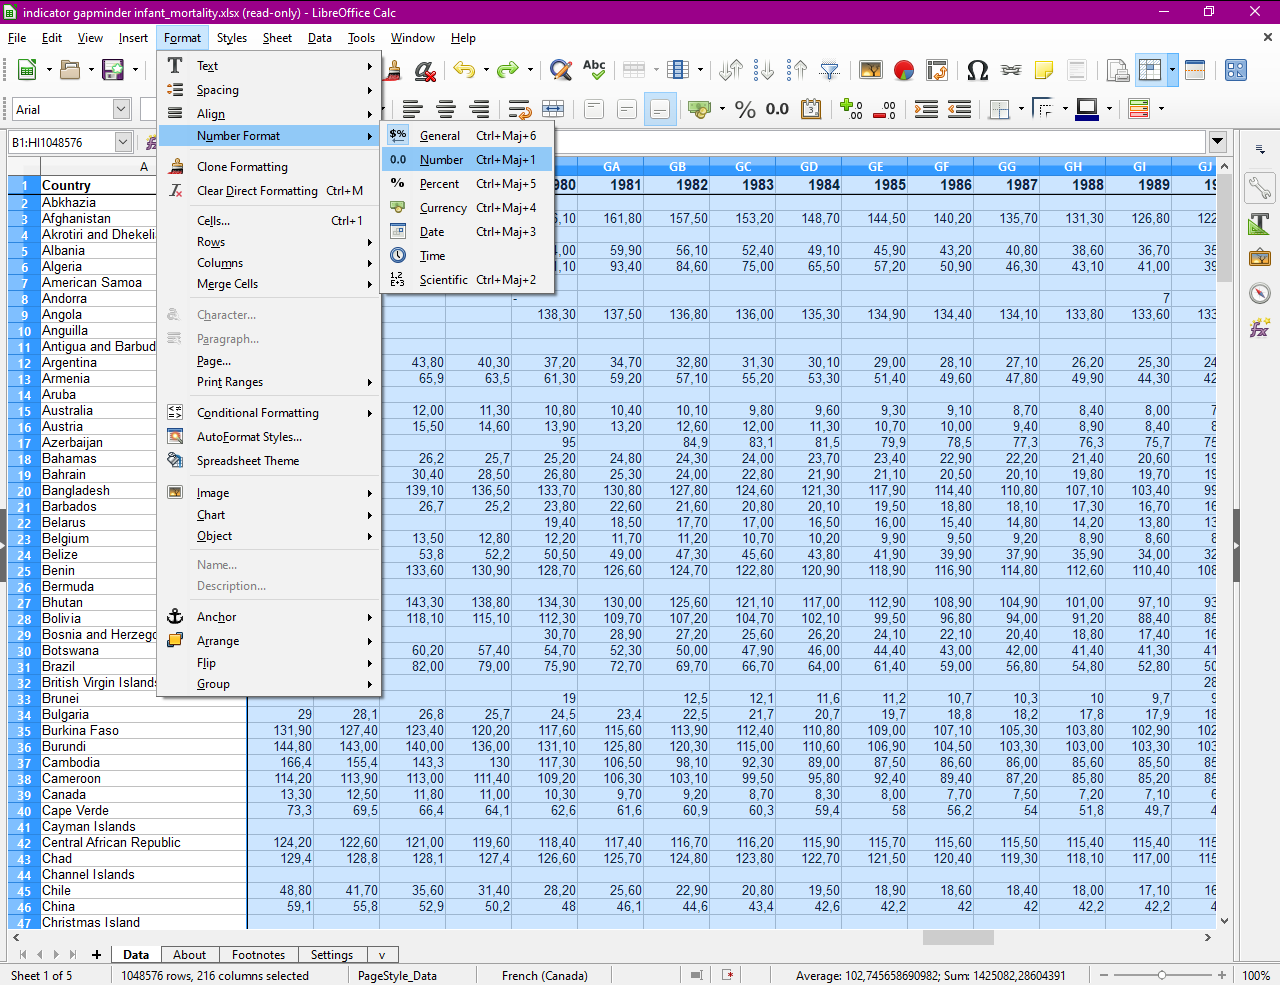
\includegraphics[width=1.0\textwidth]{format.png}
			\caption{Applying number format to selected columns in LibreOffice.}
			\label{fig:format}
		\end{figure}
	
		Once in R, import the data using \code{read.csv}. Once that is done, however, you should always doubt that everything went well. Just to prove my point, let's examine the imported data a little more closely (see section~\ref{sec:types} about data frames and section~\ref{sec:access} about the \code{\$} operator):
		\begin{minted}[breaklines]{R}
> infant = read.csv('C:/.../r-tutorial/infant.csv', header=TRUE)
> class(infant)
[1] "data.frame"
> str(infant)
'data.frame':   260 obs. of  217 variables:
$ Country: Factor w/ 260 levels "Abkhazia","Afghanistan",..: 1 ...
$ X1800  : int  NA NA NA NA NA NA NA NA NA NA ...
$ X1801  : int  NA NA NA NA NA NA NA NA NA NA ...
# ...
$ X1861  : int  NA NA NA NA NA NA NA NA NA NA ...
$ X1862  : Factor w/ 11 levels "",".","110","131",..: 1 1 1 1 ...
$ X1863  : Factor w/ 13 levels "",".","106","113",..: 1 1 1 1 ...
# ... 
		\end{minted}
		
		Wait, what? The country is of type factor, we all agree on that, but infant mortality rate for 1862 is a factor? Let's pick 1862 and see if we can't just eyeball the problem:
		\begin{minted}[breaklines]{R}
> infant$X1862
[1]      250.00
[16]     			150.00
[31] 
[46]            131.00
[61] 
[76] 163.00
[91] 
[106]
[121] 
[136] 
[151]       193.00               81.00
[166]                                                  110.00
[181] 
[196] 
[211]               175.00                    139.00
[226]                                    .
[241]
[256]                                   
Levels:  . 110.00 131.00 139.00 150.00 163.00 175.00 193.00 250.00 81.00
		\end{minted}
		
		I don't know if you can see it, or if you think it's a speck of dust on your screen, but there's a lonely dot there somewhere between lines~226 and~241. I am going to assume it means it's a missing data point, since nothing else makes sense.
		
		(In other languages, like French for instance, the decimal ``point'' is a comma, and therefore the ``comma-separated'' part of comma-separated value leads to some issues, not to mention the English thousand separator. This is why you set your data format in your spreadsheet: once the cell are properly formatted, your spreadsheet will export them sensibly into the csv.)
		
		Let's try again, this time telling \code{read.csv} that dots are missing data:
		\begin{minted}[breaklines]{R}
> infant = read.csv("C:/.../r-tutorial/infant.csv", header=TRUE, na.strings=".")
> str(infant)
'data.frame':   260 obs. of  217 variables:
$ Country: Factor w/ 260 levels "Abkhazia","Afghanistan",..: 1 2 3 5 6 7 8 9 10 11 ...
$ X1800  : num  NA NA NA NA NA NA NA NA NA NA ...
# ...
$ X1897  : num  NA NA NA NA NA NA NA NA NA NA ...
[list output truncated]
		\end{minted}
		
		This looks better, however the last line displayed is for 1897. If you're a trusting person (and you should never trust a computer), you might think everything is okay now. However, I cheated and skipped ahead and tried to use this data before and encountered another QA gem. So let's make sure to display \emph{all} the variables with a trick we will see in detail later (section~\ref{subsec:iteration}; for now let's just say it applies \code{class} to every part of \code{infant}.
		\begin{minted}[breaklines]{R}
> sapply(infant, class)
Country     X1800     X1801     X1802     X1803     X1804     X1805     X1806     X1807     X1808     X1809 
"factor" "numeric" "numeric" "numeric" "numeric" "numeric" "numeric" "numeric" "numeric" "numeric" "numeric" 
# ...
X1953     X1954     X1955     X1956     X1957     X1958     X1959     X1960     X1961     X1962     X1963 
"numeric" "numeric" "numeric" "numeric" "numeric" "numeric" "numeric"  "factor" "numeric" "numeric" "numeric" 
# ...
# See that pesky 1960?
> infant$X1960
[1]        245.00        115.40 148.20        -      208.00               59.87                20.30  37.30 
# ...
[256] 88.00  123.20 92.60               
146 Levels:  - 100.60 101.60 102.00 102.10 102.20 105.00 106.70 107.40 107.50 110.60 112.00 115.40 115.50 ... 94.00
		\end{minted}
		
		So, apparently ``-'' also means missing data? Gods forbid the authors hit a snag while importing data and their software didn't warn them something foul was afoot (like R just did to us, thank you R) and they just pasted it in the global csv without noticing. (This is why science should be in databases. Real databases. They don't let you put a dash in a number field, they just don't.)
		
		Now, \emph{finally}, we get:
		\begin{minted}[breaklines]{R}
> infant = read.csv('C:/.../r-tutorial/infant.csv', header=TRUE, na.strings=c('-', '.'))
> sapply(infant, class)
Country     X1800     X1801     X1802     X1803     X1804     X1805     X1806     X1807     X1808     X1809 
"factor" "numeric" "numeric" "numeric" "numeric" "numeric" "numeric" "numeric" "numeric" "numeric" "numeric" 
# ...
X2008     X2009     X2010     X2011     X2012     X2013     X2014     X2015 
"numeric" "numeric" "numeric" "numeric" "numeric" "numeric" "numeric" "numeric"
		\end{minted}
		
		\subsubsection{Fixed-width data: \code{read.fwf}}
		In some few cases, most often when importing data from government websites who offer them up publicly in .txt format, you will encounter fixed-width data. Delimited data uses a character (most often a comma) to signify the boundary between cells of data. Fixed-width, however, always has the same number of characters for a given field. To demonstrate, figure~\ref{fig:data} shows what csv (delimited) and fixed-width data look like side by side.
		\begin{figure}[h]
			\centering
			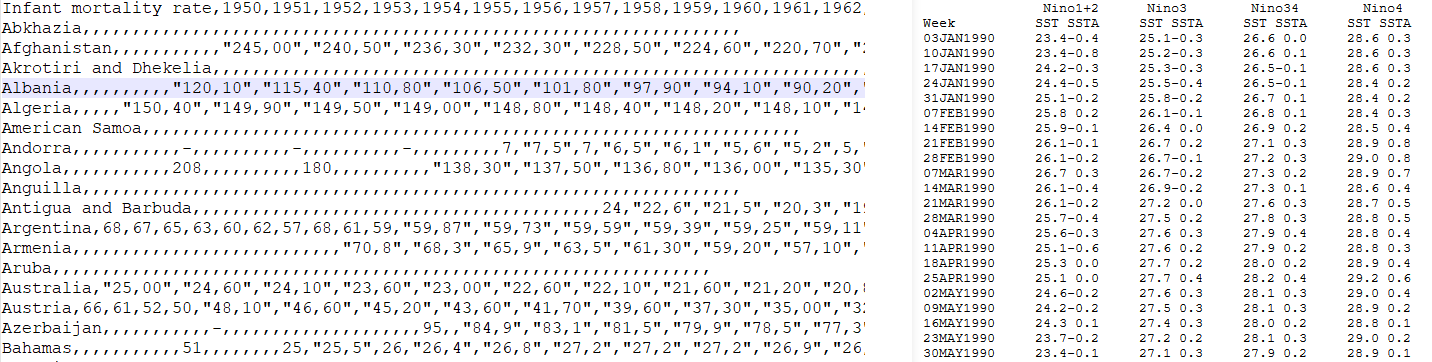
\includegraphics[width=1.0\textwidth]{data.png}
			\caption{Delimited data (left) and fixed-width data (right).}
			\label{fig:data}
		\end{figure}
		
		As a case study, let's use historic water levels for a river in Canada \cite{cehq}. Data looks like this:
		\begin{lstlisting}[breaklines, extendedchars, numbers=left]
Ministère du Développement durable, de l'Environnement et de la Lutte contre les changements climatiques
Données validées jusqu'au 1994-09-30
Station:        070401         Portneuf - à l'amont des chutes Philias                                                                                                        
Bassin versant: 3085 km2       Régime: Naturel                                           
Coordonnées:    (NAD83) 48 38' 54" // -69 10' 55"

Date de création du fichier: 2012-06-30 02:40
Particularité(s):
- 
- 
- 
Lexique:        E:  La donnée est estimée.
(Remarque)      J:  Un jaugeage a été exécuté %*à cette date.
MC: La donnée représente un débit moyen converti.
MJ: La donnée est une moyenne journalière.
P:  La donnée est provisoire.
PL: La donnée correspond %*à la premi\ère lecture de niveau d'eau de la journée.
R:  Le débit est corrigé pour tenir compte de l'effet de refoulement.
S:  La donnée est saisie manuellement.
Z:  La donnée provient d'une redistribution temporelle des données enregistrées en raison d'une défectuosité de l'appareil de mesure.

Station        Date                Débit (m3/s)   Remarque
070401         1973/08/17          86.60          J
070401         1973/08/18          79.90          MC
070401         1973/08/19          73.30          MC
070401         1973/08/20          68.80          MC
070401         1973/08/21          65.10          MC
070401         1973/08/22          63.70          MC
070401         1973/08/23          63.70          MC
070401         1973/08/24          62.00          MC
...
070401         1994/09/25          47.55          MC
070401         1994/09/26          46.74          MC
070401         1994/09/27          45.95          MC
070401         1994/09/28          46.26          MC
070401         1994/09/29          54.98          MC
070401         1994/09/30          80.23          MC
		\end{lstlisting}
		Save it as a text file on your computer as is. To read fixed-width data, you need to explicitly tell R the widths of each column. The popular Windows text editor Notepad++ shows column index, which allows to calculate them quickly: 6, 20, 15 and 12 (column starts with whitespace and ends with data). Furthermore, the ``table'' part of the file starts on line~23.
		
		(Since there are accents in the file, if you were interested in the comments, you might want to take an extracurricular dive into encodings. Since this is an English document, I will not add another painful tangent, but as a quick note, if you ever encounter trouble importing European documents, try CP-1252 (Windows default) or ISO-8859-1 (Latin extended, covers French, German and Spanish, for instance).)
		
		(Another note, there is a function to read Fortran files, which I never needed to use but might be useful to you. My condolences on dealing with Fortran.)
		
		\code{read.fwf} is used this way:
		\begin{minted}[breaklines]{R}
> debit = read.fwf("C:/.../r-tutorial/debit.txt", widths=c(6, 20, 15, 12), header=FALSE, skip=22, strip.white=TRUE, col.names=c('Station', 'Date', 'Debit', 'Remarque'))
> str(debit)
'data.frame':   7715 obs. of  4 variables:
$ Station : int  70401 70401 70401 70401 70401 70401 70401 ...
$ Date    : Factor w/ 7715 levels "1973/08/17","1973/08/18",..: 1 2 3 4 5 6 7 8 9 10 ...
$ Debit   : num  86.6 79.9 73.3 68.8 65.1 63.7 63.7 62 59.2 ...
$ Remarque: Factor w/ 5 levels "E","J","MC","R",..: 2 3 3 3 3 ...
> debit[1:5,]
Station       Date Debit Remarque
1   70401 1973/08/17  86.6        J
2   70401 1973/08/18  79.9       MC
3   70401 1973/08/19  73.3       MC
4   70401 1973/08/20  68.8       MC
5   70401 1973/08/21  65.1       MC
		\end{minted}
		
		As opposed to \code{read.csv}, I used the argument \code{header=FALSE} with \code{read.fwf}. This is due to \code{read.fwf} being pickier about the header format: it wants the header to be \emph{delimited} with a character that is not present in the rest of the file (to practice, type in \code{?read.fwf} in R and \emph{attentively} read the help about the \code{header} argument). Since this was not the case, I manually set the column names with \code{col.names}. \code{strip.white = TRUE} automatically strips the whitespace within the columns, so your date is '1973/08/17' and not '         1973/08/17'.
		
		The structure of the data frame informs us that the date as been read as a factor. Since dates are their own Pandora boxes in computer science, we will not deal with them here, but you can look at section~\ref{subsec:dates} if you're a masochist.
		
		\subsection{Export}
		Exporting data is useful to save it for later use or send to a spreadsheet software. Despite some internationalization issues, I would recommend using csv for the output file, since it is easy to import into spreadsheet software. In that simple case, the \code{write.csv} function works quite well:
		\begin{minted}[breaklines]{R}
> demo
[,1]   [,2]   [,3]   [,4]   [,5]
[1,]  82.94 115.94  89.48 101.06  91.23
[2,] 111.22 117.65  94.64 115.79 103.91
[3,]  82.10  95.96 101.11  82.44  98.84
> write.csv(demo, file='path.../demo.csv', row.names=FALSE)
		\end{minted}
		
		With data frames, the column headers will make sense and, should your object have row names, you can remove the \code{row.names} argument.
		
		\subsection{Tidy}\label{subsec:tidy}
		This section is quite heavy on R programmy-like stuff, so you may want to skip it until you are more familiar with R or actually need to disentangle a data set, whichever comes first.
		
		Since their help pages are, in my opinion, easier to understand, I use the functions in the \code{tidyr} package, so you might want to install and load it to follow along.
		
		\subsubsection{n -\textgreater 1 rows: \code{spread}}
		When the data is placed in a table where the name of a variable is used as a value in cells, you need to make them into columns. In other words, your table has a column of \emph{keys} followed by a column of \emph{values}. You can do so with the \code{spread} function, the result of which is represented in figure~\ref{fig:spread}.
		\begin{figure}[h]
			\centering
			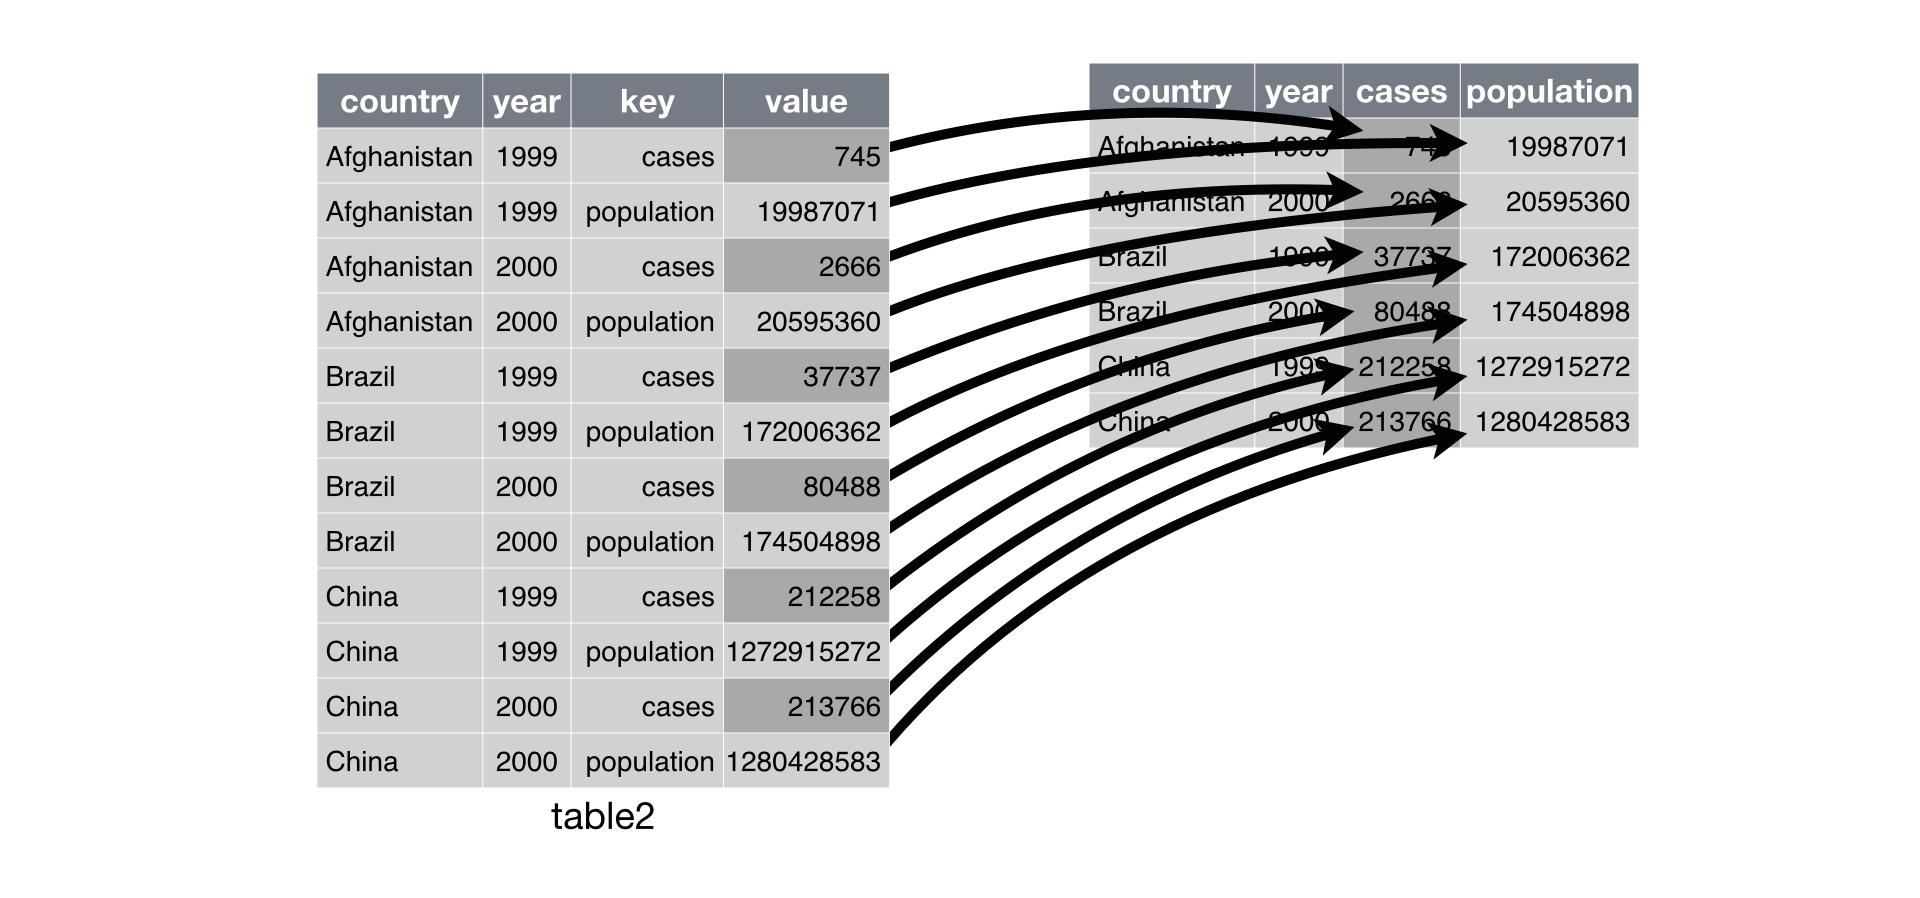
\includegraphics[width=0.8\textwidth]{spread.png}
			\caption{Putting variables in their own columns with \code{spread} (taken from \cite{tidy}).}
			\label{fig:spread}
		\end{figure}
		
		\subsubsection{1 -\textgreater n rows: \code{gather}}
		When the data is placed in a table where the column headers are values of a variable, you need to put them into one column, as shown in figure~\ref{fig:gather}. You can do so with the \code{gather} function.
		
		\begin{figure}[h]
			\centering
			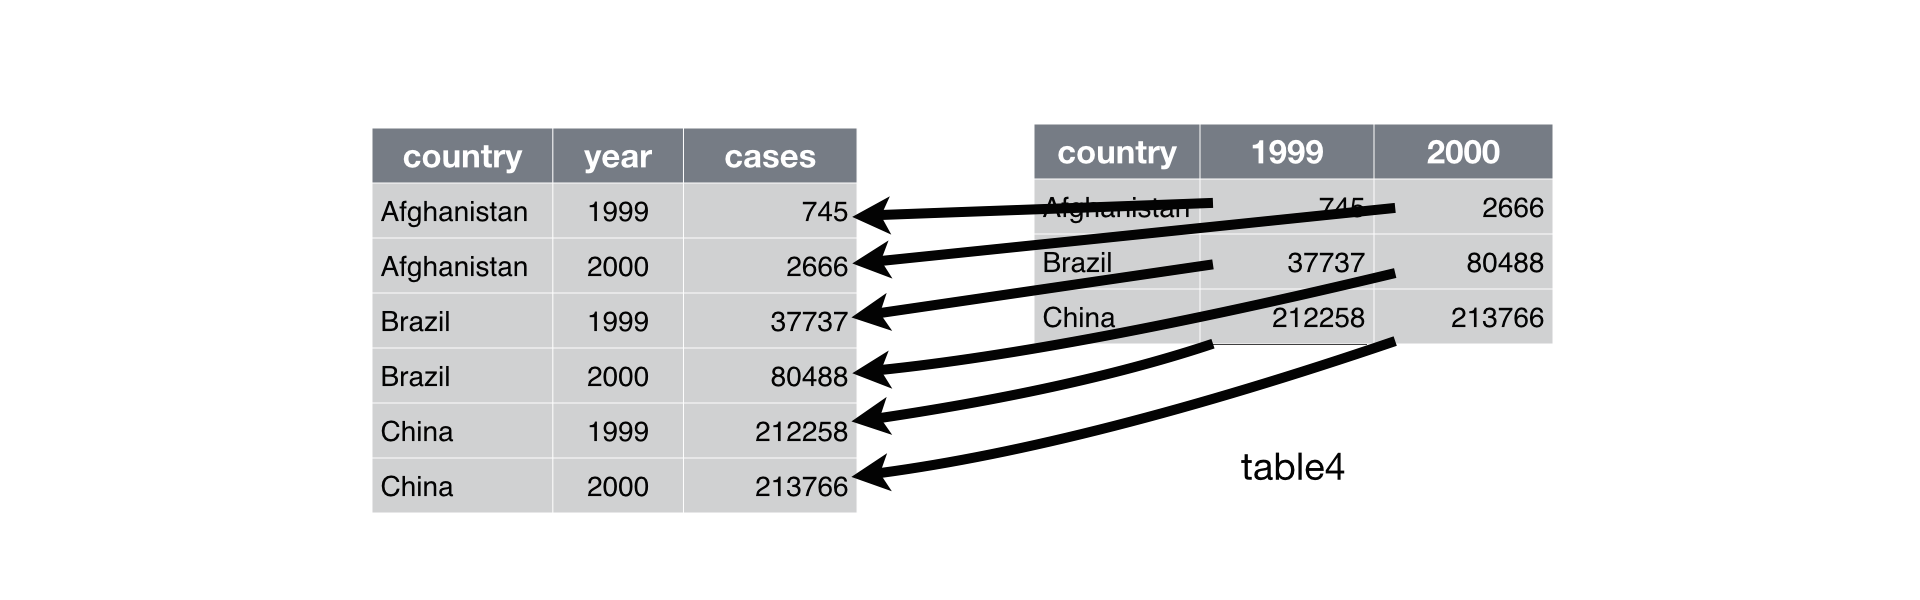
\includegraphics[width=0.8\textwidth]{gather.png}
			\caption{Putting a variable into only one column with \code{gather} (taken from \cite{tidy}).}
			\label{fig:gather}
		\end{figure}
		
		\subsubsection{1 -\textgreater n columns: \code{separate}}
		If one of the columns contain more than one variable, for example it is a rate written as cases/population, since number of cases and population are two separate variables, you will need to split this column into several others. You can use the \code{separate} function for this, as shown in figure~\ref{fig:separate}.
		
		\begin{figure}[h]
			\centering
			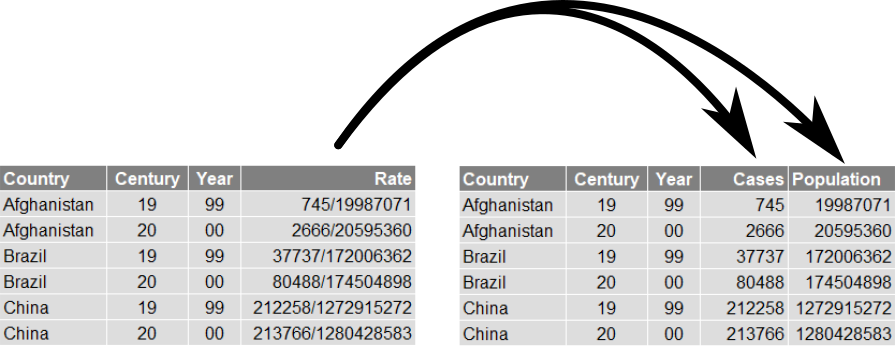
\includegraphics[width=0.8\textwidth]{separate.png}
			\caption{Separate one column into two with \code{separate} (inspired by \cite{tidy}).}
			\label{fig:separate}
		\end{figure}
		
		\subsubsection{n -\textgreater 1 columns: \code{unite}}
		If one variable is spread across multiple columns, for example a date split in year, month and day, while the date is a single variable, you will need to combine them into a single column. This can be done with the \code{unite} function, as pictured in figure~\ref{fig:unite}.
		
		\begin{figure}[h]
			\centering
			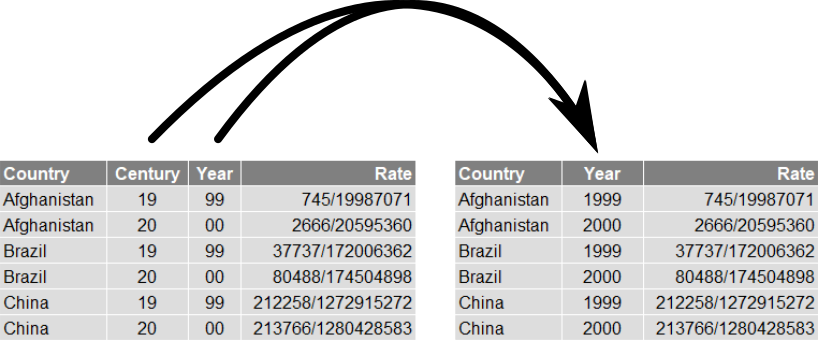
\includegraphics[width=0.8\textwidth]{unite.png}
			\caption{Merge two columns into one with \code{unite} (inspired by from \cite{tidy}).}
			\label{fig:unite}
		\end{figure}
	
		\subsubsection{Example}
		The cancer data mentioned as an example in section~\ref{subsec:gotcha_tidy} will be used as a case study for these functions. Data can most easily be copy-pasted into a Spreadsheet software from Table 1 of  the peer-reviewed article version of the report online \cite{siegel_cancer_2018}. As a first step, remove sum lines and columns, remove the thousand separator and tweak header names (also, the hyphen is not a real hyphen, so retype it). 
		
		Let's identify the variables: cancer type, sex of patient, number of cases, and number of deaths. Here, we need to make sex its own column; and since there are two columns with female data, we will proceed in several steps: first, make all four columns one ``variable'' with \code{gather}. Arguments \code{key} and \code{value} are simply the name to give to the new columns that \code{gather} will create. The last argument is the columns to ``gather'', while the columns not listed will be duplicated as necessary.
		\begin{minted}[breaklines]{R}
> cancer = read.csv('C:/.../r-tutorial/cancer.csv')
> str(cancer)
'data.frame':   47 obs. of  5 variables:
$ cancer       : Factor w/ 47 levels "Acute lymphocytic leukemia",...
$ cases_male   : int  12490 7980 14250 2440 13480 16520 ...
$ cases_female : int  4620 5600 3340 820 3810 9720 5040 ...
$ deaths_male  : int  1750 1770 2480 1280 12850 6510 810 ...
$ deaths_female: int  760 880 750 360 3000 4290 640 23240 ...
> cancer = gather(cancer, key="tmpvar", value="n", 2:5)
> str(cancer)
'data.frame':   188 obs. of  3 variables:
$ cancer: Factor w/ 47 levels "Acute lymphocytic leukemia",...
$ tmpvar: chr  "cases_male" "cases_male" "cases_male" ...
$ n     : int  12490 7980 14250 2440 13480 16520 5430 49690 ...
> cancer
    cancer        tmpvar      n
1   Tongue    cases_male  12490
2    Mouth    cases_male   7980
#...
48  Tongue  cases_female   4620
49   Mouth  cases_female   5600
#...
95  Tongue   deaths_male   1750
96   Mouth   deaths_male   1770
#...
142 Tongue deaths_female    760
143  Mouth deaths_female    880
#...
		\end{minted}
		
		Now, we need to separate the two words in the ``tmpvar'' column into two columns with \code{separate}. Arguments should be self-explanatory.
		\begin{minted}[breaklines]{R}
> cancer = separate(cancer, col="tmpvar", into=c("category", "sex"), sep="_")
> cancer
cancer category    sex      n
1    Tongue    cases   male  12490
2     Mouth    cases   male   7980
#...
48   Tongue    cases female   4620
49    Mouth    cases female   5600
#...
95   Tongue   deaths   male   1750
96    Mouth   deaths   male   1770
#...
142  Tongue   deaths female    760
143   Mouth   deaths female    880
#...
		\end{minted}
		
		Finally, we need to bring ``cases'' and ``deaths'' back as their own column with \code{spread}. The argument \code{key} is the name of the column containing the variable names that you want to make into their own column. The argument \code{value} is the name of the column whose values you want to show under the new columns to be created. Other columns will be arranged accordingly.
		\begin{minted}[breaklines]{R}
> cancer = spread(cancer, key="category", value="n")
> str(cancer)
'data.frame':   94 obs. of  4 variables:
$ cancer: Factor w/ 47 levels "Acute lymphocytic leukemia",...
$ sex   : chr  "female" "male" "female" "male" ...
$ cases : int  2670 3290 9140 10380 5620 2960 1510 1940 ...
$ deaths: int  640 830 4490 6180 680 480 660 930 7340 9490 ...
> cancer
    cancer    sex  cases deaths
#...
37   Mouth female   5600    880
38   Mouth   male   7980   1770
#...
81  Tongue female   4620    760
82  Tongue   male  12490   1750
#...
		\end{minted}
		
		Finally, let's correctly specify that ``sex'' is a \gls{qlv} rather than just text.
		\begin{minted}[breaklines]{R}
> cancer$sex = as.factor(cancer$sex)
> str(cancer)
'data.frame':   94 obs. of  4 variables:
$ cancer: Factor w/ 47 levels "Acute lymphocytic leukemia",.:...
$ sex   : Factor w/ 2 levels "female","male": 1 2 1 2 1 2 1 2 ...
$ cases : int  2670 3290 9140 10380 5620 2960 1510 1940 10160 ...
$ deaths: int  640 830 4490 6180 680 480 660 930 7340 9490 ...

		\end{minted}
		
		There we go! Tidy data set!

\chapter{Data presentation}
	\section{Frequency table (1D) or contingency table (2D)}
	\notefor{For qualitative, discrete and continuous variables}
		
	If you feel the need to make a table with your data, use a spreadsheet software. ;) R is superior in statistics and (arguably) in figures, but spreadsheets definitely have their uses when it comes to tables.
	
	\section{Pie chart}
	\notefor{For qualitative and discrete variables, max 2 values}
		
	A pie chart is a graph that can be used to visually represent proportions of a \gls{qlv} or \gls{dv}. Note that they have their critics, who recommend never using them, as our brain is bad at comparing the size of slices~\cite{wiki_pie}.
	
	As an example data set, let's use ebola deaths by country~\cite{who}. An excerpt giving the source data is shown in figure~\ref{fig:ebola}. Enter the data in your favorite spreadsheet software and save it as a csv. You should get the following:
	\begin{minted}[breaklines]{R}
Country,Deaths
Guinea,2543
Liberia,4809
Sierra Leone,3956
Mali,6
Nigeria,8
United States of America,1
	\end{minted}
	\begin{figure}[h]
		\centering
		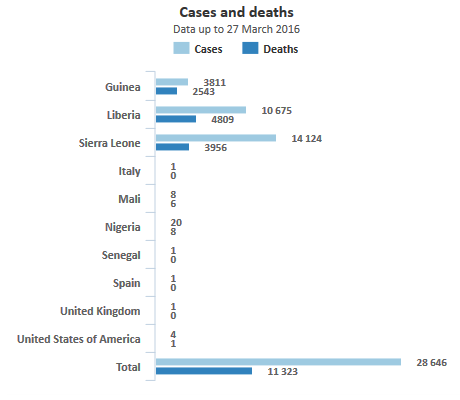
\includegraphics[width=0.8\textwidth]{ebola.png}
		\caption{Excerpt from \cite{who}.}
		\label{fig:ebola}
	\end{figure}

	Go ahead and load your small csv into R with \code{read.csv}. You can then use the function \code{pie} to produce a pie chart. However, as shown below, a naive approach might disappoint.
	\begin{minted}[breaklines]{R}
> ebola = read.csv('C:/.../r-tutorial/ebola.csv', header=TRUE)
> ebola
                   Country Deaths
1                   Guinea   2543
2                  Liberia   4809
3             Sierra Leone   3956
4                     Mali      6
5                  Nigeria      8
6 United States of America      1
> pie(ebola)
Error in pie(ebola) : 'x' values must be positive.
	\end{minted}

	You might be scratching your head and wondering which part of 2543 or 6 is not positive, and you'd be justified to do so. Here, one must dive into computer programming concerns to understand what is going on. The ``not positive'' message hints at a problem with the format or the type of the input data (see section~\ref{sec:types}). Let's demonstrate:
	\begin{minted}[breaklines]{R}
> values = c(2543, 4809, 3956, 6, 8, 1)
> labels = c('Guinea', 'Liberia', 'Sierra Leone', 'Mali', 'Nigeria', 'United States of America')
> pie(values, labels=labels)	# works! produces figure below
> class(values)
[1] "numeric"
> class(labels)
[1] "character"
> class(ebola)
[1] "data.frame"
> class(ebola$Country)
[1] "factor"
> class(ebola$Deaths)
[1] "integer"
> pie(ebola$Deaths, labels=ebola$Country)	# works too now!
	\end{minted}
	\begin{figure}[h]
		\centering
		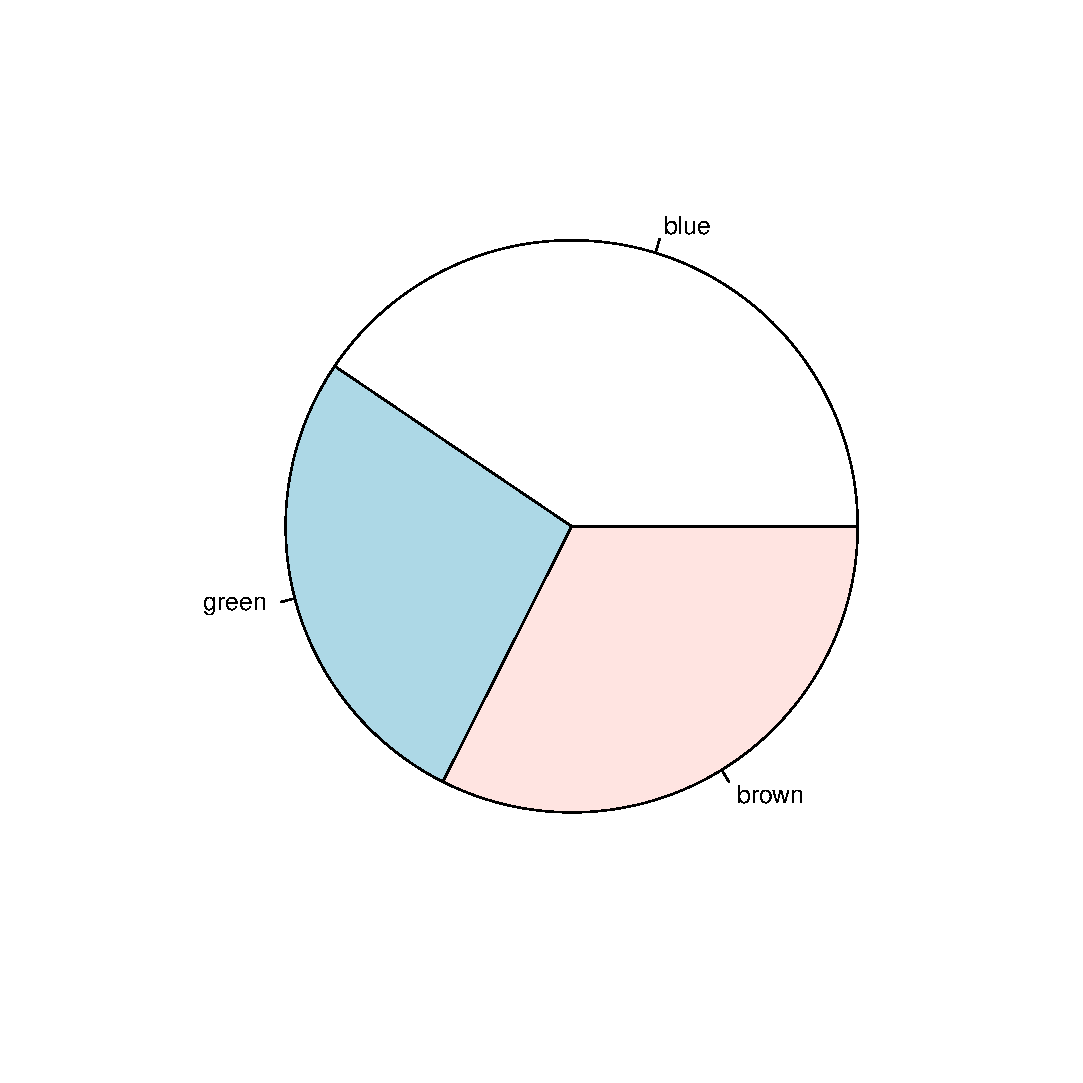
\includegraphics[width=0.8\textwidth]{pie.eps}
		\caption{Ebola deaths in 2015-2016 by country.}
	\label{fig:pie}
	\end{figure}

	Technically, \code{read.csv} returns a \code{data.frame}, while \code{pie} only accepts numbers. Accessing the columns of the data frame (see section~\ref{sec:access}) to feed \code{pie} the right types of arguments allows it to produce the expected figure.

	Now that we have our basic pie chart, you might be thinking, ``That squiggle on the right with the tiny pie slices is quite unseemly''. In addition, you might want to tweak other aspects of the graph, like adding a title or choosing colors. We will discuss common graph properties in a following section, to keep it all in the same place. As a note, all options are always listed in the function's help page.
		
	Let's just deal with the pie-chart specific problem of small slices here (I reiterate, you should run away, run away into the arms of a bar chart.), and add a percent annotation, as that is a common occurrence. R does not offer an option to deal with small slices out of the box (probably because it tells you in its own manual to use bar charts instead), so let's just manually tweak the labels:
	\begin{minted}[breaklines]{R}
> labels = as.character(ebola$Country)
> labels[4]='Others'
> labels[5:6]=''
> labels
[1] "Guinea"       "Liberia"      "Sierra Leone" "Others"       ""            
[6] ""
> percents = ebola$Deaths/sum(ebola$Deaths)*100
> percents
[1] 22.458712355 42.471076570 34.937737349  0.052989490  0.070652654
[6]  0.008831582
> percents[4] = sum(percents[4:6])
> percents
[1] 22.458712355 42.471076570 34.937737349  0.132473726  0.070652654
[6]  0.008831582
> percents = round(percents, 2)
> percents
[1] 22.46 42.47 34.94  0.13  0.07  0.01
> labels[1:4] = paste(labels[1:4], percents[1:4], '%')
> labels
[1] "Guinea 22.46 %"       "Liberia 42.47 %"      "Sierra Leone 34.94 %"
[4] "Others 0.13 %"
> pie(ebola$Deaths, labels)
	\end{minted}
	Hacky, but it works, and no more time should be dedicated to pie charts, so let's move on.

	\section{Bar chart}
	\notefor{For qualitative and discrete variables}
		
	A bar chart, sometimes called a line graph, is used to represent a \gls{qlv} or a \gls{dv}, and the bars \emph{do not touch}. As an example, data on infant mortality by country can be found at \href{https://docs.google.com/spreadsheets/d/1OHMMuHbSFKDolNHXsmgHYlkjSKfAZyyY1P-ddMu_Fz0/pub}{Gapminder}~\cite{gapminder}. The import process is detailed in section~\ref{subsec:import}.

	A barplot is relatively straightforward to produce with R, but we will see all ``common'' (imho) plot options here, so tie your winter hat down with wire, you'll be sitting here a while.  Let's start by simply plotting infant mortality rate by country. To keep the plot readable, let's choose a subset of G8 countries: Canada, France, Germany, Italy, Japan, Russia, United Kingdom and United States of America. Let's also start by studying the mortality rate in 2000. First, we will select each of the countries by its row number, then we will stitch the G8 back together with a function called \code{rbind}, which binds data frames together by row, as long as all data frames have the same columns.
	\begin{minted}[breaklines]{R}
> canada = infant[38,]
> france = infant[77,]
> germany = infant[83,]
> italy = infant[109,]
> japan = infant[111,]
> russia = infant[186,]
> uk = infant[240,]
> usa = infant[241,]
> g8 = rbind(canada, france, germany, italy, japan, russia, uk, usa)
	 \end{minted}

	Producing a barplot now is easy:
	\begin{minted}[breaklines]{R}
> barplot(g8$X2000, names.arg=g8$Country)
	\end{minted}
	\begin{figure}[h]
		\centering
		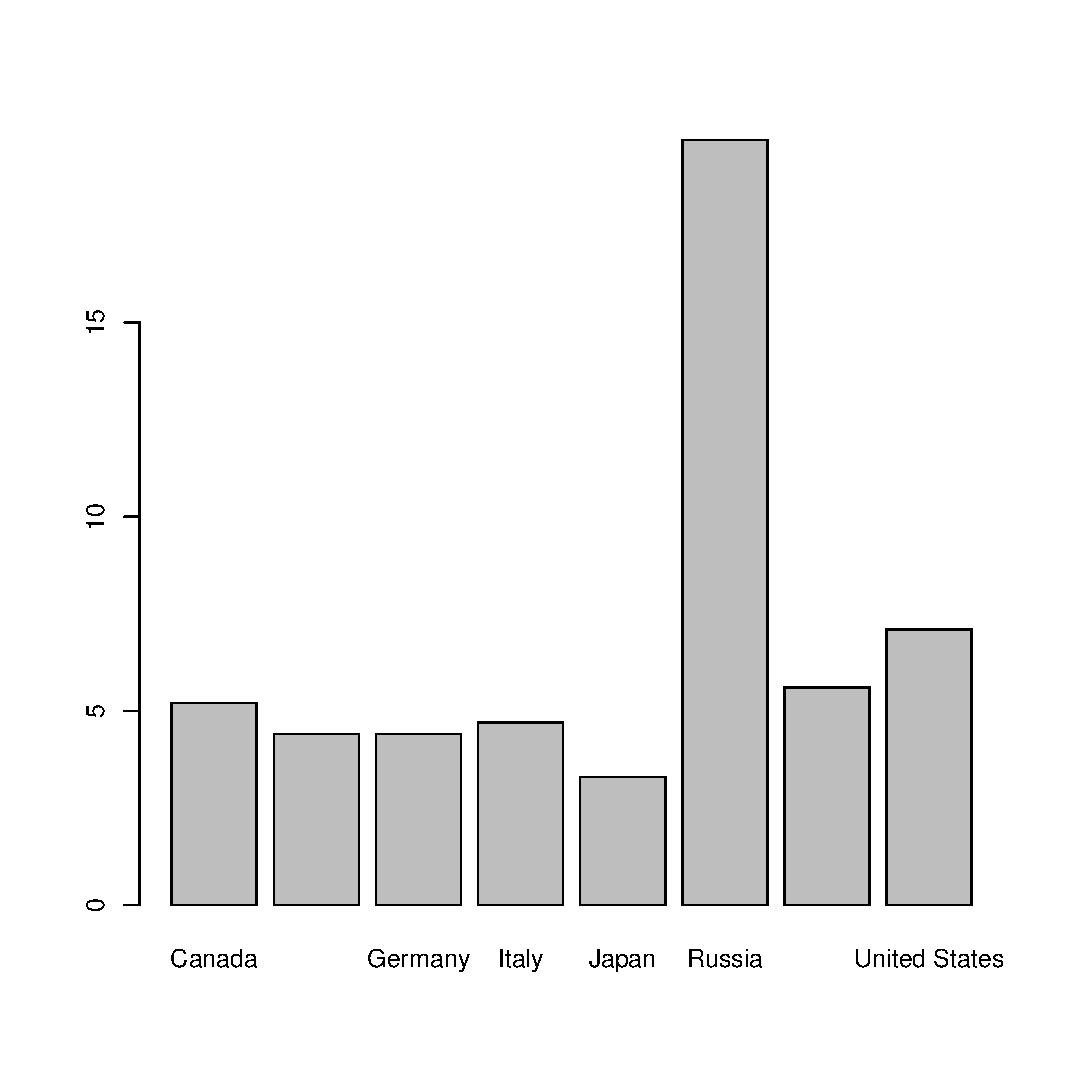
\includegraphics[width=1.0\textwidth]{barsimple.eps}
		\caption{Simplest bar plot: infant mortality rate per country.}
	\label{fig:simplebar}
	\end{figure}

	Several things are wrong with this graph. Glaringly, a bar should not extend beyond its axis. Axes are set as plot options with \code{xlim} and \code{ylim}. Also, should you want a box around the graph, \code{bty} takes care of that. Usually. Bar plots are special and you need to all an extra function after your plot appears. See all graph options with \code{?par}, which we will use a lot more as we customize our graphs.
	\begin{minted}[breaklines]{R}
> barplot(g8$X2000, names.arg=g8$Country, ylim=c(0,20), bty='o')	
> # why oh why won't bty work like everywhere else!
> box()
	\end{minted}
	\begin{figure}[h]
		\centering
		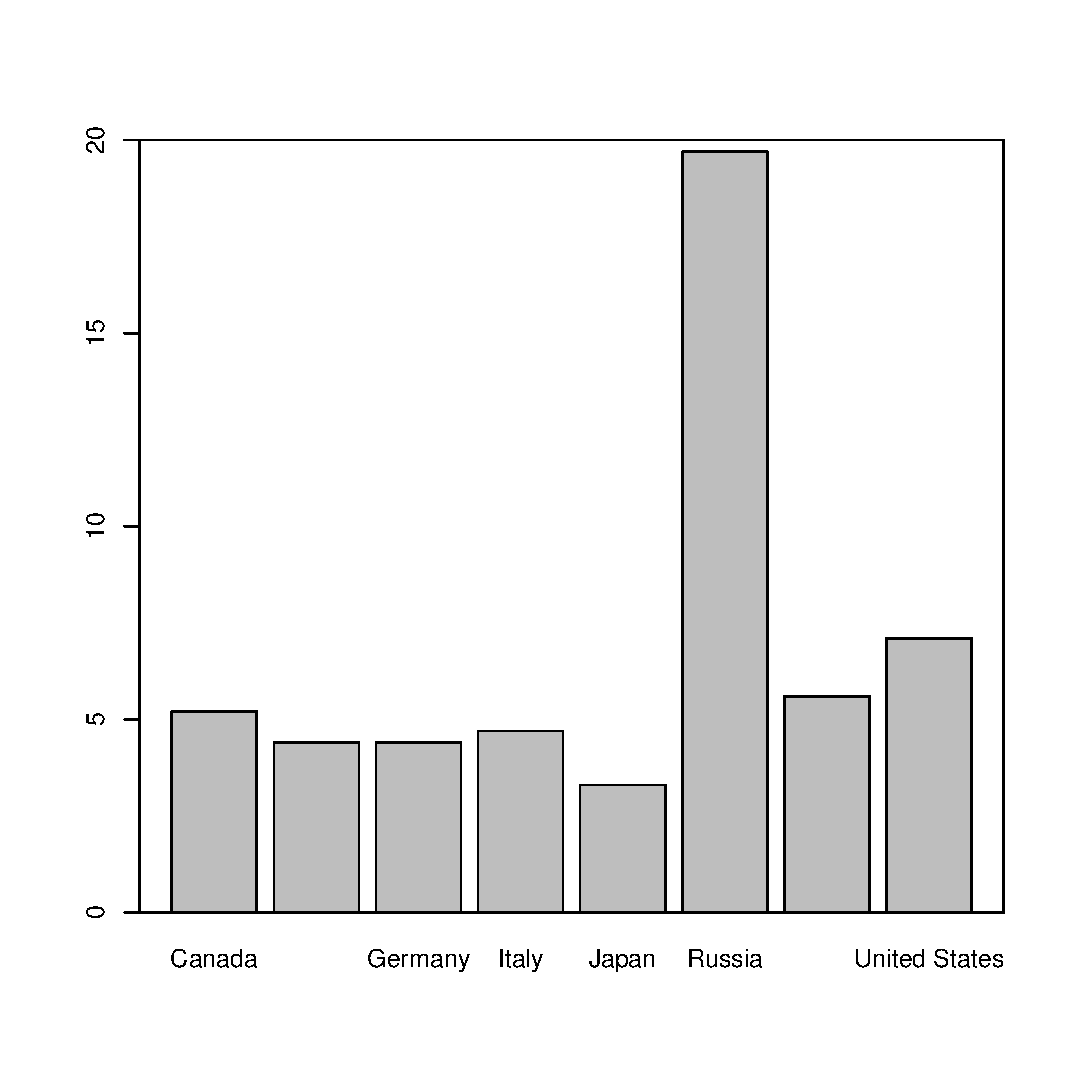
\includegraphics[width=1.0\textwidth]{baraxis.eps}
		\caption{Simple bar plot: infant mortality rate per country, axis set.}
		\label{fig:baraxis}
	\end{figure}

	You probably also want all country names to show up. Easiest way to do that is to tilt the axis label text. Here we will learn about \code{par}, used \emph{before} your graph function to specify general plotting settings. For this next iteration, let's do a few things at once. First, let's make all labels perpendicular to their axis with \code{par} and \code{las}. Let's also demonstrate color manipulation by making each country's bar the dominant color on their flag (I may have made some arbitrary choices) with \code{col}.
	\begin{minted}[breaklines]{R}
> colors = c('red', 'blue', 'black', 'green', 'white', 'snow', 'purple', 'purple4')
> par(las=2)		# axis labels: perpendicular
> barplot(g8$X2000, names.arg=g8$Country, ylim=c(0,20), col=colors)
> box()
	\end{minted}

	\begin{tcolorbox}[title=Colors in R, parbox=false]
Colors in R can be specified by their names, if they are among R's list of predefined colors, which you can see by calling \code{colors()}.

A more visually helpful version can be found at \href{http://research.stowers.org/mcm/efg/R/Color/Chart/}{Color Chart}~\cite{rcolors} which, incidentally, has other fascinating references about the use of color in science (good vs. bad color ramps, color blindness, etc).

Additionally, colors can be specified in other formats like \code{\#RRGGBB}. These values can be found with graphics software or off a color generator on the internet.

Finally, if color space is a concern, additional functions exist: \code{rgb}, \code{hsv}, \code{hcl}, \code{gray} and \code{rainbow}.
	\end{tcolorbox}

	\begin{figure}[h]
		\centering
		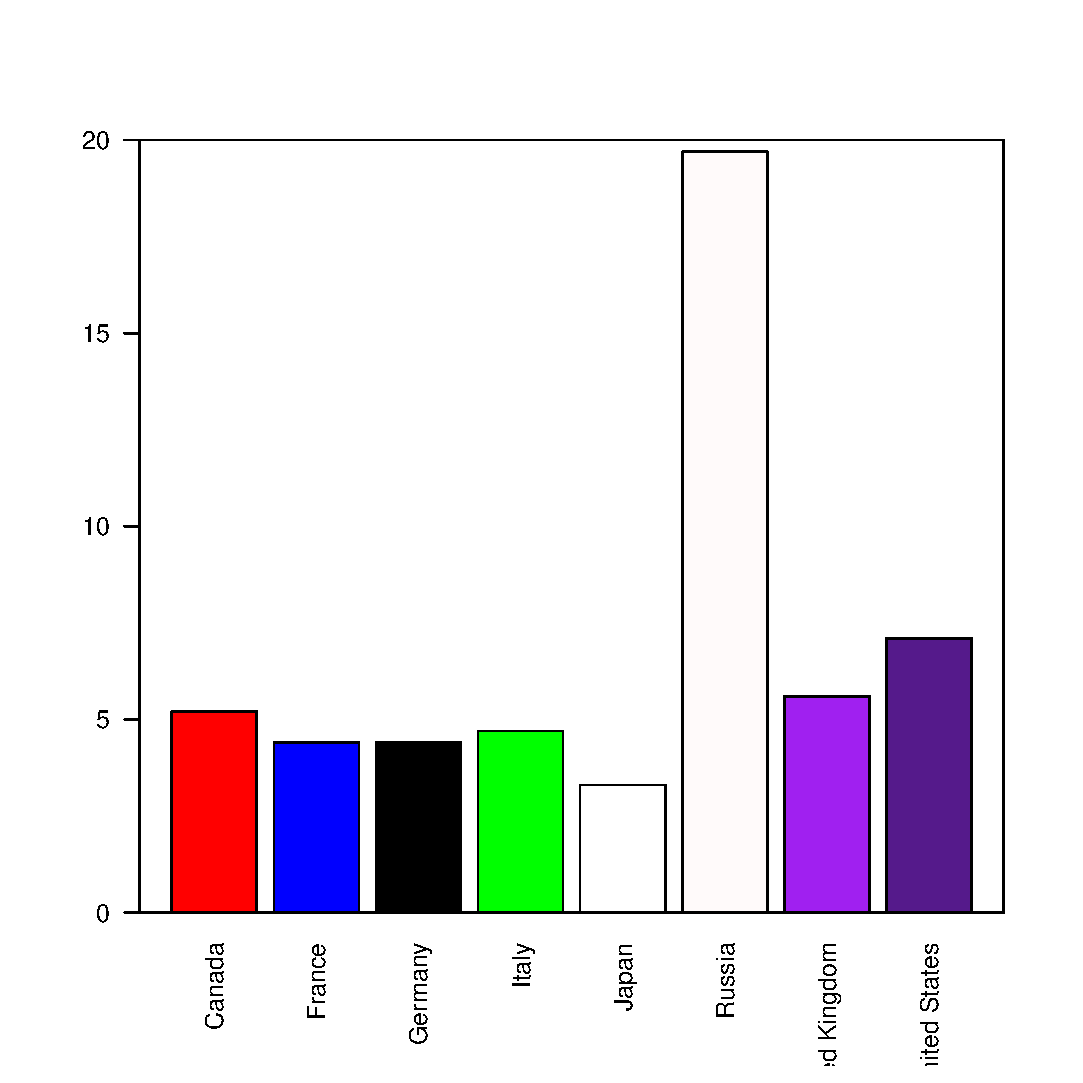
\includegraphics[width=1.0\textwidth]{barpsych.eps}
		\caption{Psychedelic bar plot: infant mortality rate per country, axis set, labels perpendicular, colors.}
		\label{fig:barpsych}
	\end{figure}

	With the country names printed at the vertical, they are running out of space at the bottom of the graph. More margin is needed there. Figures have two types of margins in R: outer and inner. The inner margin is used to draw the figure title and the axis ticks and labels and can be set in inches with \code{mai=c(bottom, left, top, right)} or in lines with \code{mar=c(bottom, left, top, right)}. The outer margin is outside the figure; it makes more sense when several plots are displayed together, as we will do a few exercises down the line. The outer margin as well can be set in inches with \code{omi=c(bottom, left, top, right)} or in lines with \code{oma=c(bottom, left, top, right)}. As for the appropriate margin necessary to display the full country name, that's a matter of trial and error. Starting with the current parameters' value of inner margin, I found that a value of 8 worked well.
	\begin{minted}[breaklines]{R}
par()$mar
[1] 5.1 4.1 4.1 2.1
> # mar = c(bottom, left, top, right)
> par(mar=c(8, 4.1, 4.1, 2.1))
> barplot(g8$X2000, names.arg=g8$Country, ylim=c(0,20), col=colors)
> box()
	\end{minted}

	Now, bar charts often use stacked bars. For example, let's use cancer rates \cite{cancer}. This data includes number of cases and number of deaths by sex and cancer type. If the thing you would most like to compare is the number of cancer by type, you would stack the sexes into one bar. Let's use the tidy version of the data set produced in section~\ref{subsec:tidy}.
	\begin{minted}[breaklines]{R}
> str(cancer)
'data.frame':   94 obs. of  4 variables:
$ cancer: Factor w/ 47 levels "Acute lymphocytic leukemia",.:...
$ sex   : Factor w/ 2 levels "female","male": 1 2 1 2 1 2 1 2 ...
$ cases : int  2670 3290 9140 10380 5620 2960 1510 1940 10160 ...
$ deaths: int  640 830 4490 6180 680 480 660 930 7340 9490 ...
	\end{minted}
	The help page of \code{barplot} tells you that the first argument can be either a \code{vector} or \code{matrix}. If \code{height} is a \code{vector}, for example the single column \code{cancer\$deaths}, then the barplot shows what one would expect. If \code{height} is a \code{matrix}, then each \emph{column} must be either the values to stack (\code{beside=FALSE}) or the values for a group of bars (\code{beside=TRUE}). To visualize, let's plot data for five short-named cancers in the list. And since this is a perfect occasion, let's learn about a few more figure options: the \code{legend} argument and how to plot several figures into one plot window.
	\begin{minted}[breaklines]{R}
> subset=rbind(cancer[11:12,], cancer[17:18,], cancer[35:36,], cancer[63:64,], cancer[79:80,])
> subset = subset[, 1:3] 
> subset
     cancer    sex  cases deaths
11   Breast female 266120  40920
12   Breast   male   2550    480
17    Colon female  47530  23240
18    Colon   male  49690  27390
35 Melanoma female  36120   3330
36 Melanoma   male  55150   5990
63  Pharynx female   3340    750
64  Pharynx   male  14250   2480
79  Thyroid female  40900   1100
80  Thyroid   male  13090    960
> fordemo = spread(subset[, 1:3], cancer, cases) # let's just use cases for now
> fordemo
sex Breast Colon Melanoma Pharynx Thyroid
1 female 266120 47530    36120    3340   40900
2   male   2550 49690    55150   14250   13090
> # each column of the matrix is one cancer to stack or group
> str(fordemo)
'data.frame':   2 obs. of  6 variables:
$ sex     : Factor w/ 2 levels "female","male": 1 2
$ Breast  : int  266120 2550
$ Colon   : int  47530 49690
$ Melanoma: int  36120 55150
$ Pharynx : int  3340 14250
$ Thyroid : int  40900 13090
> # but you want an actual matrix, not a data frame
> # with row and column names
> # and cells containing numbers only
> fordemo = as.matrix(fordemo[,2:6])
> fordemo
Breast Colon Melanoma Pharynx Thyroid
[1,] 266120 47530    36120    3340   40900
[2,]   2550 49690    55150   14250   13090
> rownames(fordemo) = c("female", "male")
> fordemo
       Breast Colon Melanoma Pharynx Thyroid
female 266120 47530    36120    3340   40900
male     2550 49690    55150   14250   13090
\end{minted}
	
	At this point, your data is ready in the shape that \code{barplot} wants it: it's a matrix with each column representing a stack or group. It's also in the shape \emph{you} want it because the row and column names are readable. Now, let's use \code{mfrow} to plot the results of \code{beside=TRUE} and \code{beside=FALSE} side by side, as seen in figure~\ref{fig:mfrow}.
	\begin{minted}[breaklines]{R}
> par(mfrow=c(1,2))   # 1 row, 2 columns, fill by row
> # par(mfcol=c(1,2)) # 1 row, 2 columns, fill by column
> # a plot window opens, ready with 1x2 plot regions
> barplot(fordemo, beside=FALSE, legend=TRUE, main="Parameter beside=FALSE")
> # first plot appears on the left
> barplot(fordemo, beside=TRUE, legend=TRUE, main="Parameter beside=TRUE")
> # second plot appears on the right
	\end{minted}
	
	\begin{figure}[h]
		\centering
		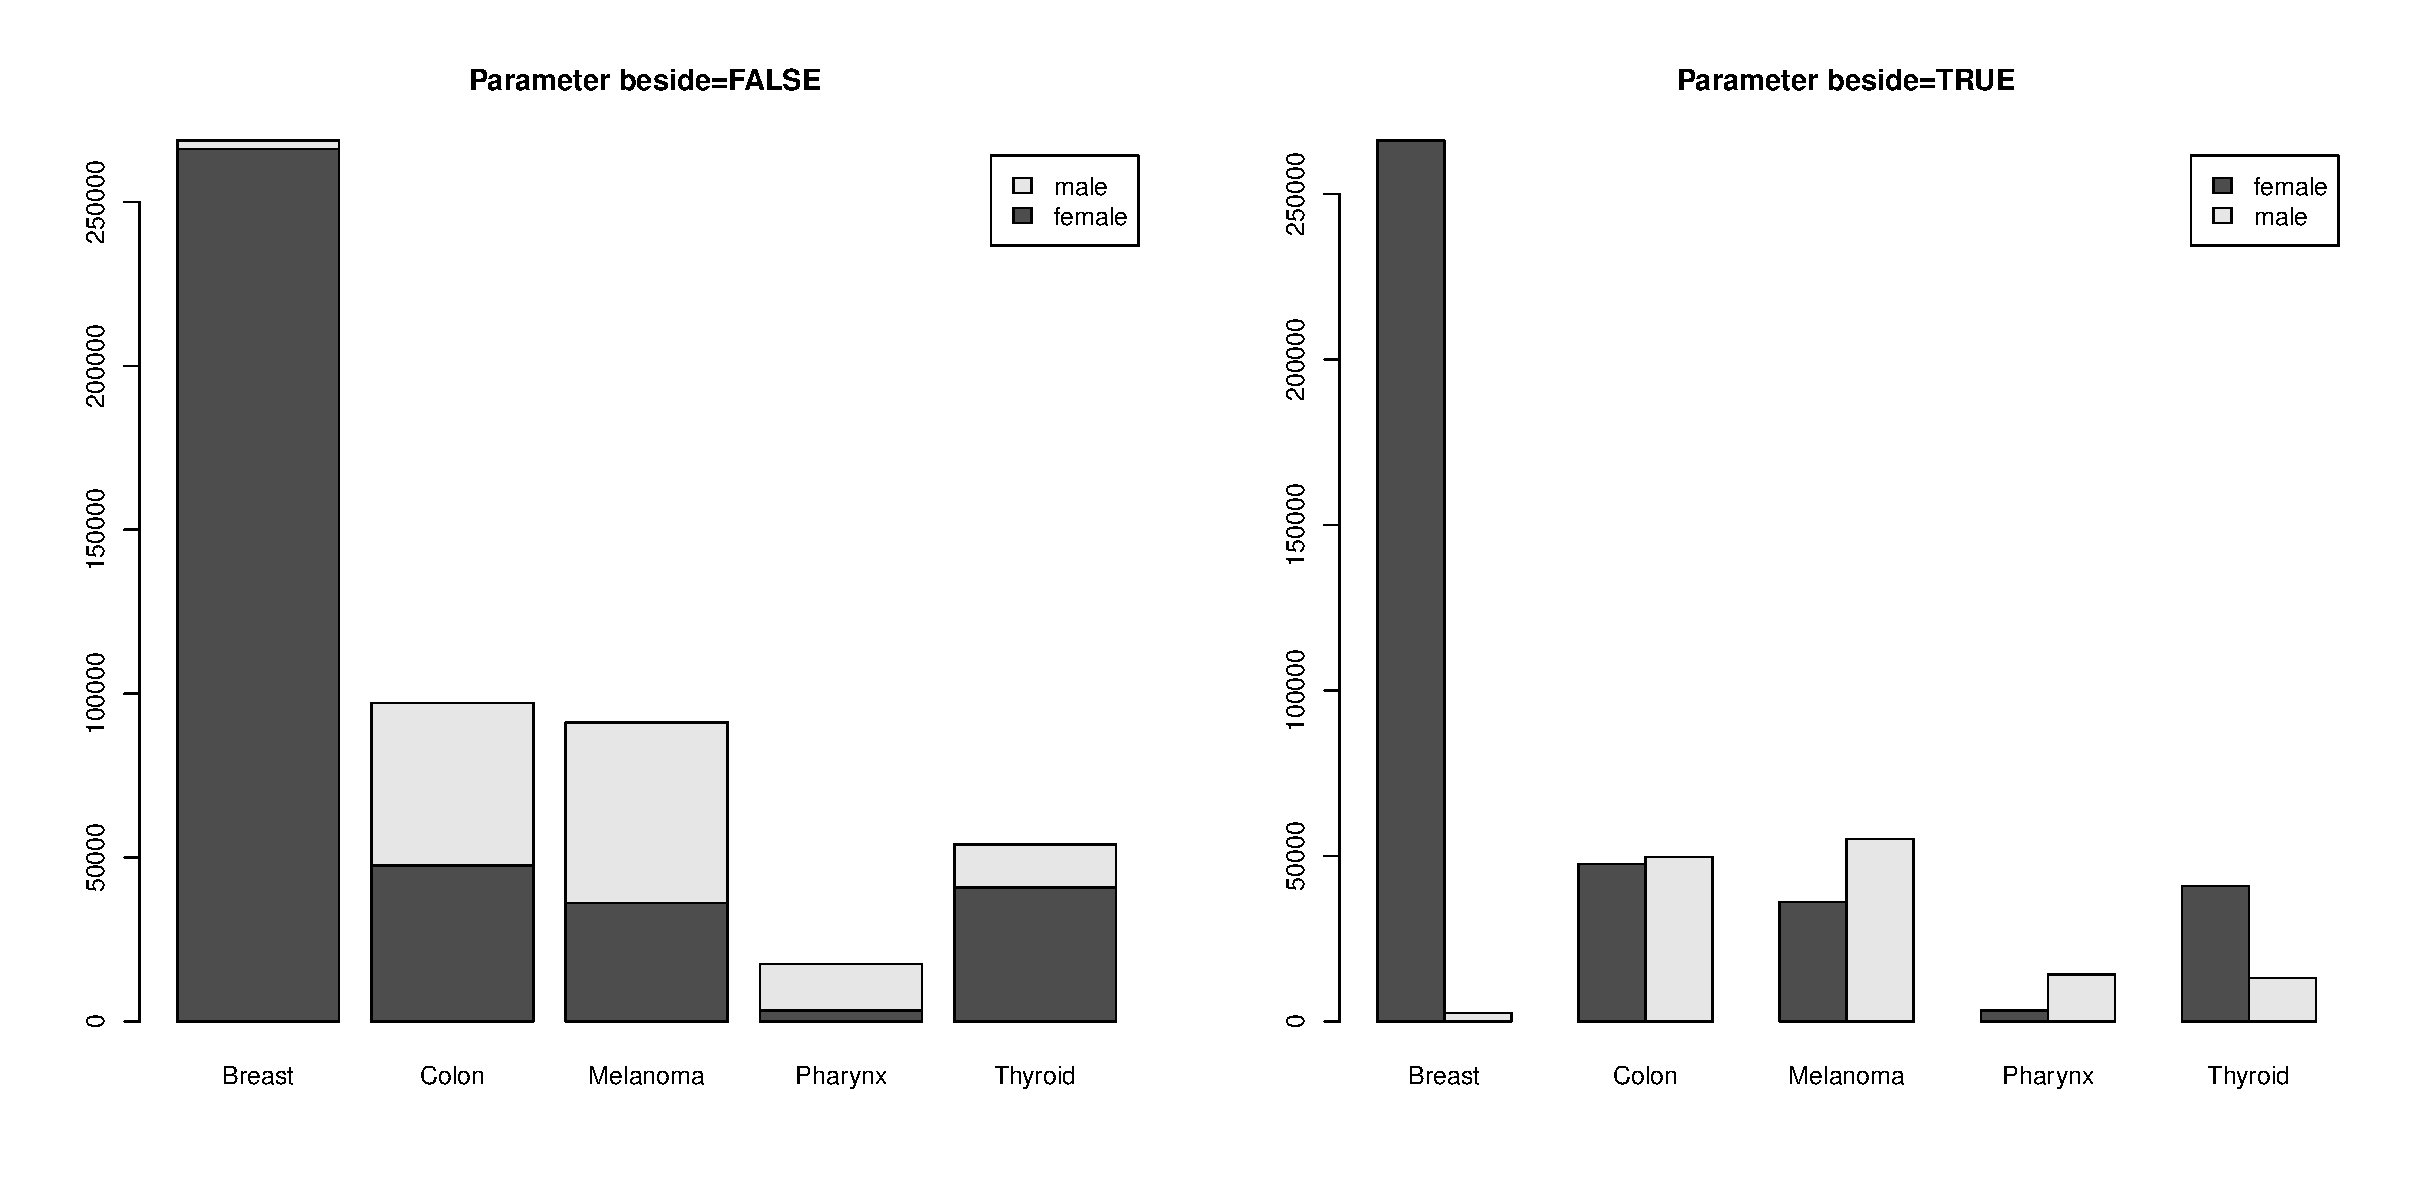
\includegraphics[width=1.0\textwidth]{mfrow.eps}
		\caption{Comparing the effect of the \code{beside} parameter for a matrix fed to \code{barplot}, using \code{mfrow}.}
		\label{fig:mfrow}
	\end{figure}

	Note that setting the \code{legend} argument automatically produces a human-readable result from the row names of the ``fordemo'' matrix.
	
	Now, if you want to stack sexes and group cases and deaths per cancer, this is where \code{barplot} would fail you and you would have to resort to a package, for example \code{ggplot2}. According to discussions in the R mailing lists, the basic bar plot function does not support this option because the developers felt it was too much information to fit on one figure, so keep that in mind and ask yourself whether it's a good idea. However, as shown by the pie chart section, I'm not here to judge, so here's a way to do that.
	
	\code{ggplot2} is so ubiquitously used to produce peer-review quality graphics in R, while being so different from the basic graphics we have used so far that it warrants a bit of an introduction.
	
	\code{ggplot2} works by sequentially adding \emph{layers} from a \emph{data frame}. So first, you say, ``I want to make a new \code{ggplot}''. An empty graphics window opens. Then you say, ``I want to add points to this blank canvas''. Then you can say, ``I want to add a line in addition to the points already there'', and then ``I also want a main title'', and so on. So you will add new function calls separated by a plus sign.
	
	With our cancer study case, our situation is that we want to stack sexes, as well as group cases and deaths (which we will call effect) per cancer. You need each of these in their own column, and you need a data frame since that's what \code{ggplot} uses. Our data must be transformed this way:
	\begin{minted}[breaklines]{R}
> forgg = gather(subset, "effect", "n", 3:4)
> forgg
cancer    sex effect      n
1    Breast female  cases 266120
2    Breast   male  cases   2550
3     Colon female  cases  47530
4     Colon   male  cases  49690
5  Melanoma female  cases  36120
6  Melanoma   male  cases  55150
7   Pharynx female  cases   3340
8   Pharynx   male  cases  14250
9   Thyroid female  cases  40900
10  Thyroid   male  cases  13090
11   Breast female deaths  40920
12   Breast   male deaths    480
13    Colon female deaths  23240
14    Colon   male deaths  27390
15 Melanoma female deaths   3330
16 Melanoma   male deaths   5990
17  Pharynx female deaths    750
18  Pharynx   male deaths   2480
19  Thyroid female deaths   1100
20  Thyroid   male deaths    960
\end{minted}
	
	As for the plotting part of the work, \code{ggplot} loves to use scientific notation, so we'll turn that off. \code{ggplot} comes with several ``themes'', which control a series of layout options like background color, presence of grids, etc. We'll use the classic theme since it looks most like the basic graphics package we have been using.
	\begin{minted}[breaklines]{R}
options(scipen=999)
theme_set(theme_classic())
	\end{minted}
	
	\code{ggplot}'s first argument is the source data frame. Then, you will need to specify what it calls an \emph{aesthetic}: what do you want to show in x and y? We want our variable ``n'' to be shown as y, and we want ``effect'' and ``cancer'' on x.
	
	This leads me to talk of \emph{facets} and \emph{formulas}. Facets are a \code{ggplot2} thing, while formulas are used throughout R. So basically, we want to divide our graph into several smaller graphs, one for each type of cancer, and show them side by side. So each "subgraph" is a facet. Therefore, we will use ``cancer'' in the facet function, and it leaves ``effect'' as the x in the \code{ggplot}'s aesthetic.
	
	As for formulas, they define a more ``talkative'' way for you to specify which relationship you want R to study for you. The most basic form is \code{y \textasciitilde x}, which reads ``y as a function of x''. More elaborate forms include \code{y + z \textasciitilde x}, which is ``y and z as a function of x'' (note, the plus sign means ``and'', not a literal addition), and \code{y \textasciitilde x | a}, which is ``y as a function of x, per value of a''.
	
	With this preliminary knowledge, we are ready to look at the code, which produces figure~\ref{fig:ggplot}.
	\begin{minted}[breaklines]{R}
> ggplot(forgg, aes(effect, n)) +		
		# use data frame forgg, x=effect, y=n
	geom_col(aes(fill=sex)) +		
		# draw columns, fill them according to sex
	facet_wrap(~cancer, nrow=1) +	
		# subdivide as a function of cancer, on 1 row
	coord_cartesian(ylim = c(0, 300000)) +	
		# adjust y axis limits
	scale_fill_manual(values = c("female"="#FF5577", "male"="#0000FF"))
		#set specific colors
	\end{minted}
	\begin{figure}[h]
		\centering
		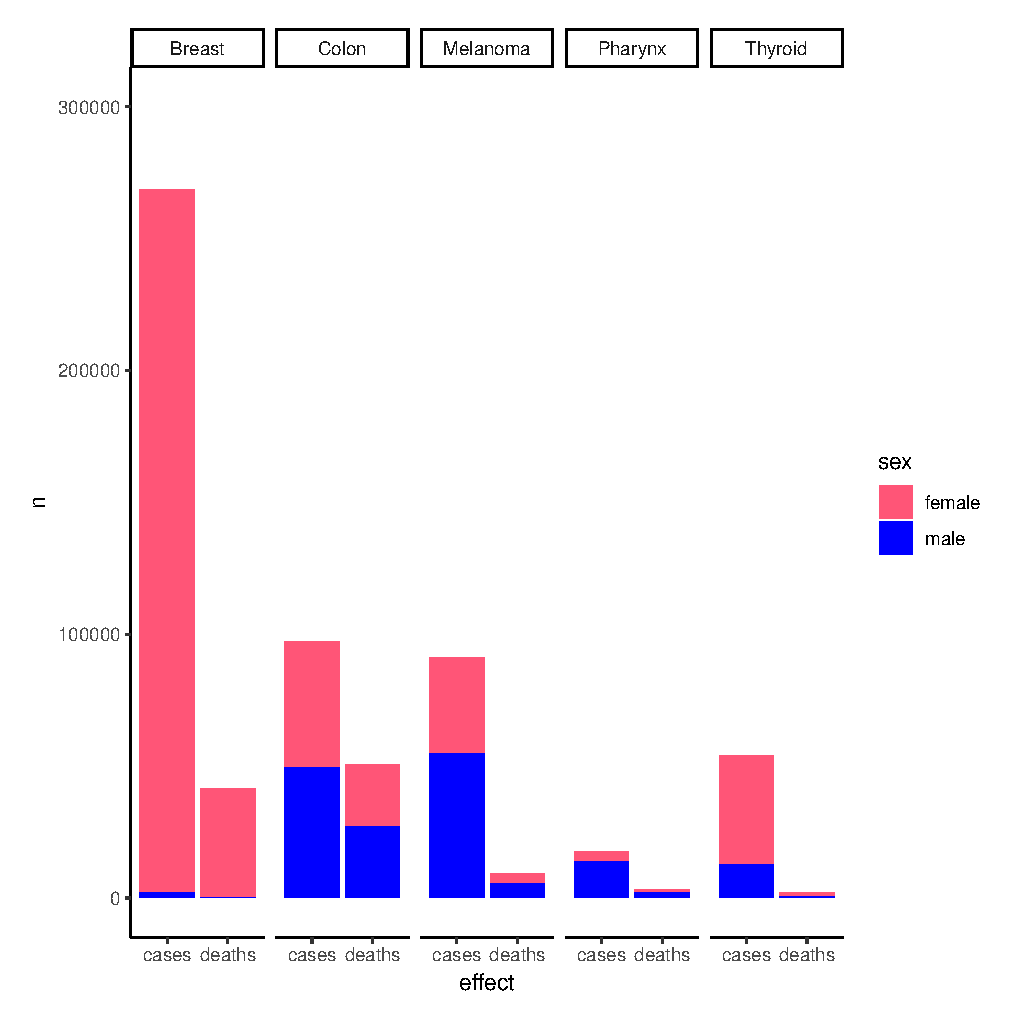
\includegraphics[width=1.0\textwidth]{ggplot.eps}
		\caption{Number of cases and deaths by sex for five cancers, with the help of \code{ggplot}.}
		\label{fig:ggplot}
	\end{figure}
	
	Your options of types of plots include: \code{geom\_point} for points, \code{geom\_col} for bars showing heights, \code{geom\_bar} for bars showing counts.
	
	You can control color and size of points, as well as fill of bars, by setting the appropriate options in the aesthetic, for example:
	\begin{minted}[breaklines]{R}
geom_point(aes(size=population, col=state))
geom_col(aes(fill=sex))
	\end{minted}
	As you may have noted when we made our figure, the legend appears automatically, with the colors and sizes (if relevant) used.
	
	You can use \code{facet\_wrap} to make your "subgraphs" follow one after the other, or \code{facet\_grid} to have them form a grid, for instance, see the code below, which produces figure~\ref{fig:facet_grid}. As for layout options regarding colors, titles, annotations, etc, they are so numerous that I can't detail them here. Digging into the help pages and asking the internet how to do things is the way to go.
	\begin{minted}[breaklines]{R}
> ggplot(forgg, aes(effect, n)) +
	geom_col(aes(fill=sex)) +
	facet_grid(cancer~sex, ) +
	scale_fill_manual(values = c("female"="#FF5577", "male"="#0000FF"))
	\end{minted}
	\begin{figure}[h]
		\centering
		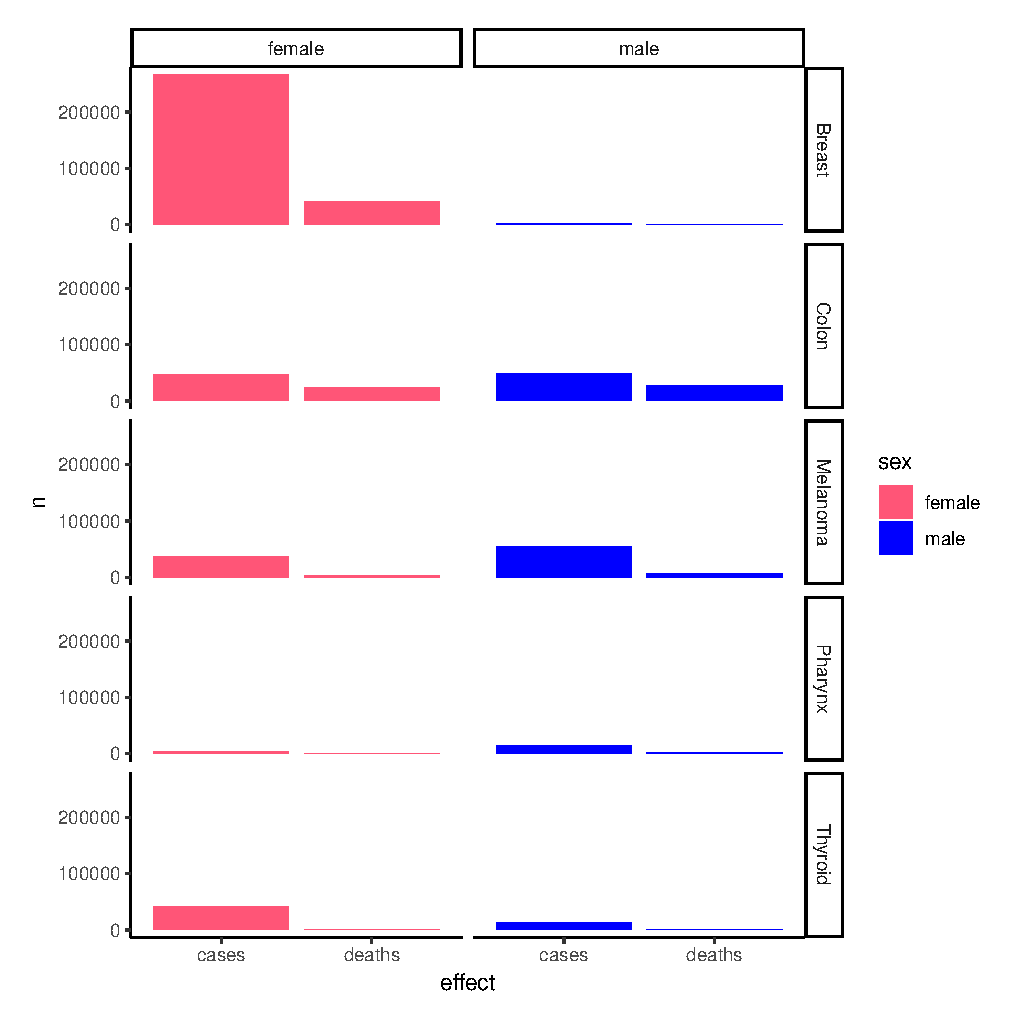
\includegraphics[width=1.0\textwidth]{facet_grid.eps}
		\caption{Grid presentation of number of cases and deaths per cancer per sex.}
		\label{fig:facet_grid}
	\end{figure}

	\section{Histogram}
	\notefor{For continuous variables}
	
	A histogram is a representation of a \gls{cv}, and \emph{the bars touch}. It is used to visually present the shape of the distribution by compiling counts for ``bins'', ranges of values. Bins are typically, but not necessarily, of equal width.
	
	For our example, let's use traffic data in the city of Chicago \cite{traffic}. 
	
	\begin{minted}[breaklines]{R}
> traffic = read.csv("C:/.../r-tutorial/traffic.csv")
> str(traffic)
'data.frame':   1279 obs. of  9 variables:
$ ID       : Factor w/ 1279 levels "1","1,000","1,001",..: 453...
$ Address  : Factor w/ 1203 levels "1 West","10 East",..: 212 ...
$ Street   : Factor w/ 251 levels "100th St","101st St",..: 40 ..
$ Date     : Factor w/ 95 levels "1/24/2007","1/30/2007",..:54...
$ Volume   : int  14600 16500 18200 21600 18300 8600 10000 ...
$ Direction: Factor w/ 1223 levels "East Bound: 1000 / West Bound: 3400",..: 397 442 484 20 495 257 939 936 981 909 ...
$ Latitude : num  41.8 41.8 41.8 41.8 41.8 ...
$ Longitude: num  -87.7 -87.7 -87.6 -87.6 -87.6 ...
$ Location : Factor w/ 1276 levels "(41.651861, -87.54501)",...
	\end{minted}
	
	
	\section{Scatter graph}
	\section{Box and whiskers graph}
	
\chapter{Data description}
	\section{Center tendency measurements}
		\subsection{Mean}
		\subsection{Median}
		\subsection{Mode}
	\section{Dispersion measurements}
		\subsection{Range}
		\subsection{Variance}
		\subsection{Standard deviation}
		\subsection{Coefficient of variation}
		\subsection{Quartiles and percentiles}
	\section{Shape measurements}
		\subsection{Skewness}
		\subsection{Kurtosis}
		\subsection{L-moments}

\chapter{Probabilities}
	\section{Factorial}
	\section{Combinations}
	\section{Permutations}
	\section{Probability Mass/Density Function}

\chapter{Statistics}
	\section{Binomial distribution}
	\section{Multinomial distribution}
	\section{Poisson distribution}
	\section{Inverse binomial distribution}
	\section{Hypergeometric distribution}
	\section{Normal distribution}
	\section{Exponential distribution}
	\section{Gamma distribution}
	\section{c2 distribution}
	\section{Fisher-Snedecor distribution}
	\section{Student’s law}

\chapter{Inferential statistics}
	\section{Student’s test}
	\section{Student’s paired test}
	\section{Bartlett’s test}
	\section{Single-factor ANOVA}
	\section{c2 test}
	\section{Wilcoxon-Mann-Whitney test}
	\section{Kolmogorov-Smirnov test}
	\section{Kruskal-Wallis test}
	\section{Pearson’s test}
	\section{Spearman’s test}
	\section{Kendall’s test}
	\section{Simple linear regression}
	\section{Multiple linear regression}

\chapter{Programming}
	\section{Sequence, iteration, branching}
		\subsection{Iteration}\label{subsec:iteration}
		\subsection{Branching}\label{subsec:branching}
	\section{Functions}
	\section{Misc}
		\subsection{Dates}\label{subsec:dates}
\chapter{Cheat sheet}

	\section{Plumbing}
\begin{tabbing}
?~~~~~~~~~~~~~ \= ?exact\_function\_name \\
?? \> ??keyword \\
class \> class(R\_variable) \\
str \> str(R\_variable) \\
colnames \> colnames(R\_variable) \\
as.integer \> as.integer(R\_variable) \\
rbind \> rbind(var, var...) \\
cbind \> cbind(var, var...)
\end{tabbing}

	\section{Data import and export}
\begin{tabbing}
read.csv~~~~ \= read.csv('delimited\_data.csv', header=TRUE, sep=",", dec=".") \\
read.fwf \> read.fwf('fixed\_width\_data.txt', widths=c(10, 5, 4), header=FALSE, skip=2, strip.white=TRUE, col.names=c('first', ...)) \\
write.csv \> write.csv(R\_variable, file='desired\_file\_name.csv', row.names=FALSE, append=FALSE)
\end{tabbing}

\printbibliography

\printnoidxglossaries

\end{document}